\documentclass[11pt,dvipdfmx]{ujarticle}
\usepackage{eee,scalefnt,graphicx}
\bibliography{3rd_diode}
\begin{document}

\begin{jikkenTitle}
 \gakunen{3} 
 \numTitle{2}{ダイオードを用いた半導体の基本的性質の検証} 
 \subTitle{(Semiconductor's basic nature verification using diode)}
 \jikkenbi{令和04年06月02日(木)} 
 \jikkenbiII{令和04年06月09日(木)} 
 \kyoudou{3301青木柊人,3305市川 潤} 
 \kyoudouII{3317杉山 滉太,3326塚原 秀翔} 
 \yoteibi{06/16}
 \yoteibiII{06/23}
 \yoteibiIII{06/30}
 \hanNumberName{1}{3309}{大山 主朗} 
\end{jikkenTitle}

\section{目的}
今回の実験では以下の3点を目的とする.
\begin{itemize}
	\item ダイオードの原理を知り,実験により整流作用を理解することでダイオードを使用できるようにする.
	\item ツェナーダイオードの特性を学び,ツェナーダイオードを使用できるようにする.
	\item 太陽電池の特性を知り,使用できるようにする.
\end{itemize}

\section{原理}
\subsection{LabVIEW}
NATIONAL INSTRUMENTS(NI)が提供しているLabVIEWは,各種計測器やmyRIOなどを用いて自動計測や制御を実装するためのグラフィカルユーザーインターフェイスのプログラミング言語である.
主な特徴は,ビルトインされた仮想計測器(Virtual Instruments,以下VI)で,オシロスコープやマルチメーターなどの計測器と似た外観や機能をコンピューター上へ作成するというものである.
VIは,フロントパネル,ブロックダイアグラム,アイコン-コネクタという3つ主要素から構成される.
プログラミングは,ブロックダイアグラム上にアイコンを配置し,各アイコン間のコネクタをつなぐ形で行う.

\subsection{myRIO}
myRIOは,デュアルコアのARM Cortex-A9 リアルプロセッサとカスタマイズ可能なXilinx FPGA・アナログプロセッサの駆動するプログラミング言語には,LabVIEWを用いる.
LabVIEWとmyRIOを用いることにより,制御,ロボット,メカトロニクス,組込などを容易に実現することができる.

\subsection{myRIO ブレッドボードアクセサリ}
myRIOの拡張ポートに接続可能なブレッドボードアクセサリ.
myRIOの5V,3.3V,GND端子及びAnalog I/O,Digital I/Oの端子が,ブレッドボード上に結線した回路とヘッダにマッピングされている.
そのため,ブレッドボード上に結線した回路とヘッダとをジャンパ線で結線することにより,回路への入出力制御および計測がmyRIOを用いて容易に実行することができる.

\subsection{可変抵抗器(ポテンショメータ)\cite{23r234r2}}
可変抵抗器(Potentiometer)は抵抗値を変更できる抵抗器の一種で,機械的な位置の変化をアナログ電気信号に変換することができる.
つまみを回すことにより,\wfig{ALPS}のように抵抗体の長さが変化することにより,抵抗値の変更が可能となっている.

\begin{figure}[h]
\centering
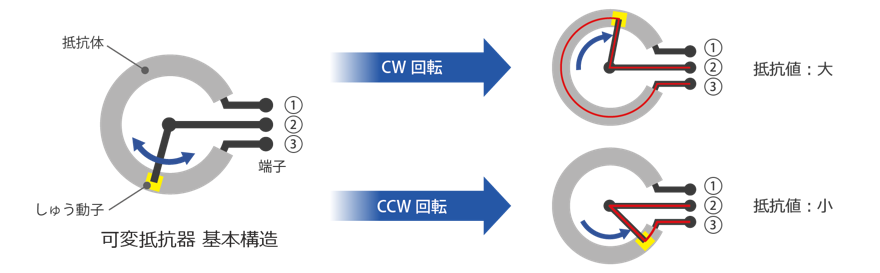
\includegraphics[scale=0.5]{/Users/ohyamasan/Downloads/TMCIT-Report/EE_Measurement/fig/pote_lp_01_02.png}
\caption{可変抵抗器の原理}
\label{fig:ALPS}
\end{figure}

\subsection{CdSセンサ\cite{dsfase}\cite{8347ty34i}\cite{B056}\cite{R300000001-I023994699-00}}
\label{CDSG}
光可変抵抗器ともいう.光電効果(photoelectric effect)である光導電性を利用し,光の強さで抵抗値が変化するCdS(硫化カドミウム)の性質を利用した電子部品.
光導電性は半導体の表面に光を当てるとキャリアが増加し,抵抗率が下がる現象である.
そのため,セルに当たる光が多ければ,抵抗値は低くなる.
赤外線や可視光線や紫外線など、広範囲の周波数にも反応するため,明るさセンサーや街の街灯のスイッチング等に用いられる.

\subsection{力センサ\cite{asdfsa}\cite{canon}}
\label{PG}
感圧センサともいう.
特殊導電部材(ゴム・フィルム)と電極で構成される.\wfig{weight}のように,接触の圧力に応じて特殊導電部材と電極の接触面積が増減することにより,抵抗値が変わる.センサ部分は円形などで,感圧エリアが決まっている.
圧力を加えていない時でも一定の抵抗値を有しており,圧力を加えると接触電極面が増加することから,抵抗値は減少する.

\begin{figure}[h]
\centering
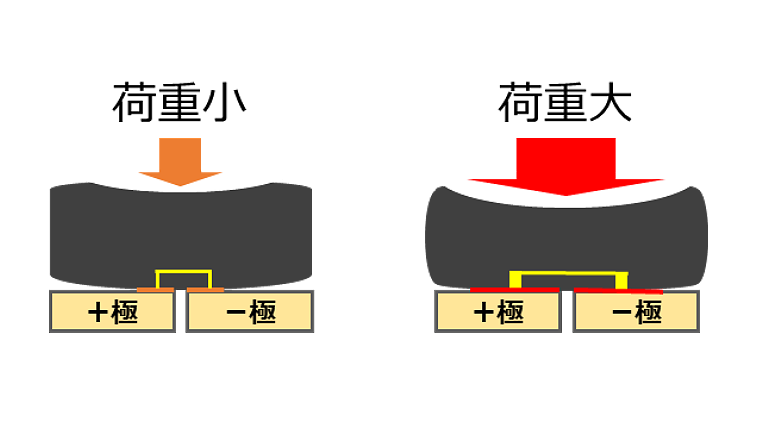
\includegraphics[scale=0.45]{/Users/ohyamasan/Downloads/TMCIT-Report/EE_Measurement/fig/sensor-03.png}
\caption{力センサの原理}
\label{fig:weight}
\end{figure}

\subsection{発光ダイオード\cite{dafadsav}\cite{gjkdgfbn}}
\label{LEDG}
LED(Light Emitting Diode)ともいう.
pn接合でできている.順方向の電圧を加えることにより,再結合エネルギーが光になって放出される.
電気エネルギーを直接光エネルギーに変換できるため,従来の光源と比べてエネルギー効率が高い.
白色LEDは\wfig{aokiro}のように,青色LED+黄色蛍光体(現在主流)のものと,\wfig{rgb}のように,赤色LED+緑色LED+青色LEDで作るものなどがある.

\begin{figure}[h]
  \begin{minipage}[]{0.5\hsize}
    \centering
    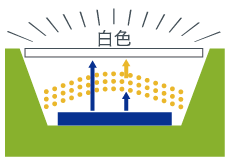
\includegraphics[scale=0.8]{/Users/ohyamasan/Downloads/TMCIT-Report/EE_Measurement/fig/led_what3_jp1.png}
    \caption{青色+黄色蛍光体手法}
    \label{fig:aokiro}
  \end{minipage}
  \begin{minipage}[]{0.5\hsize}
    \centering
    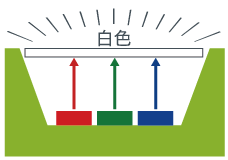
\includegraphics[scale=0.8]{/Users/ohyamasan/Downloads/TMCIT-Report/EE_Measurement/fig/led_what3_jp2.png}
    \caption{赤色+緑色+青色手法}
    \label{fig:rgb}
  \end{minipage}
\end{figure}


\subsection{真値と誤差及び相対誤差(誤差率)\cite{1130000797667922816}}
\subsubsection{真値(true value)}
真値とは,測定量(測定値ではない)が単位の何倍であるのかを示している値である.
真値は必ず存在すると仮定しても我々は真値そのものは知ることができず,ただその存在する範囲を推定することが出来るだけである.
そのため誤差は正負の符号を持っているが,それを確定することができない.
\subsubsection{誤差及び相対誤差}
測定値(measured value)及び,誤差(error)はそれぞれ,\weq{keisoku},\weq{gosa}で定義される.
\begin{align}
	測定値 &= 倍数 \times 単位\label{eq:keisoku}\\
	誤差 &= 測定値 − 真値\label{eq:gosa}
\end{align}
また,相対誤差(relative error)とは真値に対する誤差の比である.
但し真値は不明なことが多いため,通常は\weq{soutaigosa}のように誤差が小さいとして真値の代わりに測定値で割る.
\begin{eqnarray}
	相対誤差 = \frac{誤差}{真値} \fallingdotseq \frac{誤差}{測定値}
	\label{eq:soutaigosa}
\end{eqnarray}
相対誤差を百分率などで表した値を誤差率と呼ぶ.
また,以上のことから\weq{hutasikasa}のように表すこともできることがわかる\cite{1130000797042387712}.
\begin{eqnarray}
	測定値=真値 \pm 誤差=真値(1\pm 相対誤差)
\label{eq:hutasikasa}
\end{eqnarray}

\subsection{統計処理(正規分布・平均値・標準偏差)}
\subsubsection{正規分布(normal distribution)\cite{1130848328216058496}\cite{6602}}
左右対称の釣鐘型(平均値から離れるにつれて個数が減る)に値が分布している分布で,山の頂点に平均値がくる.
\wfig{normal-fig}は横軸に測定量,縦軸に正規分布の確率密度関数(probability density function)をプロットしたものである.
全体の面積(全確率)は\weq{int-nor}より1である.

\begin{figure}
\centering
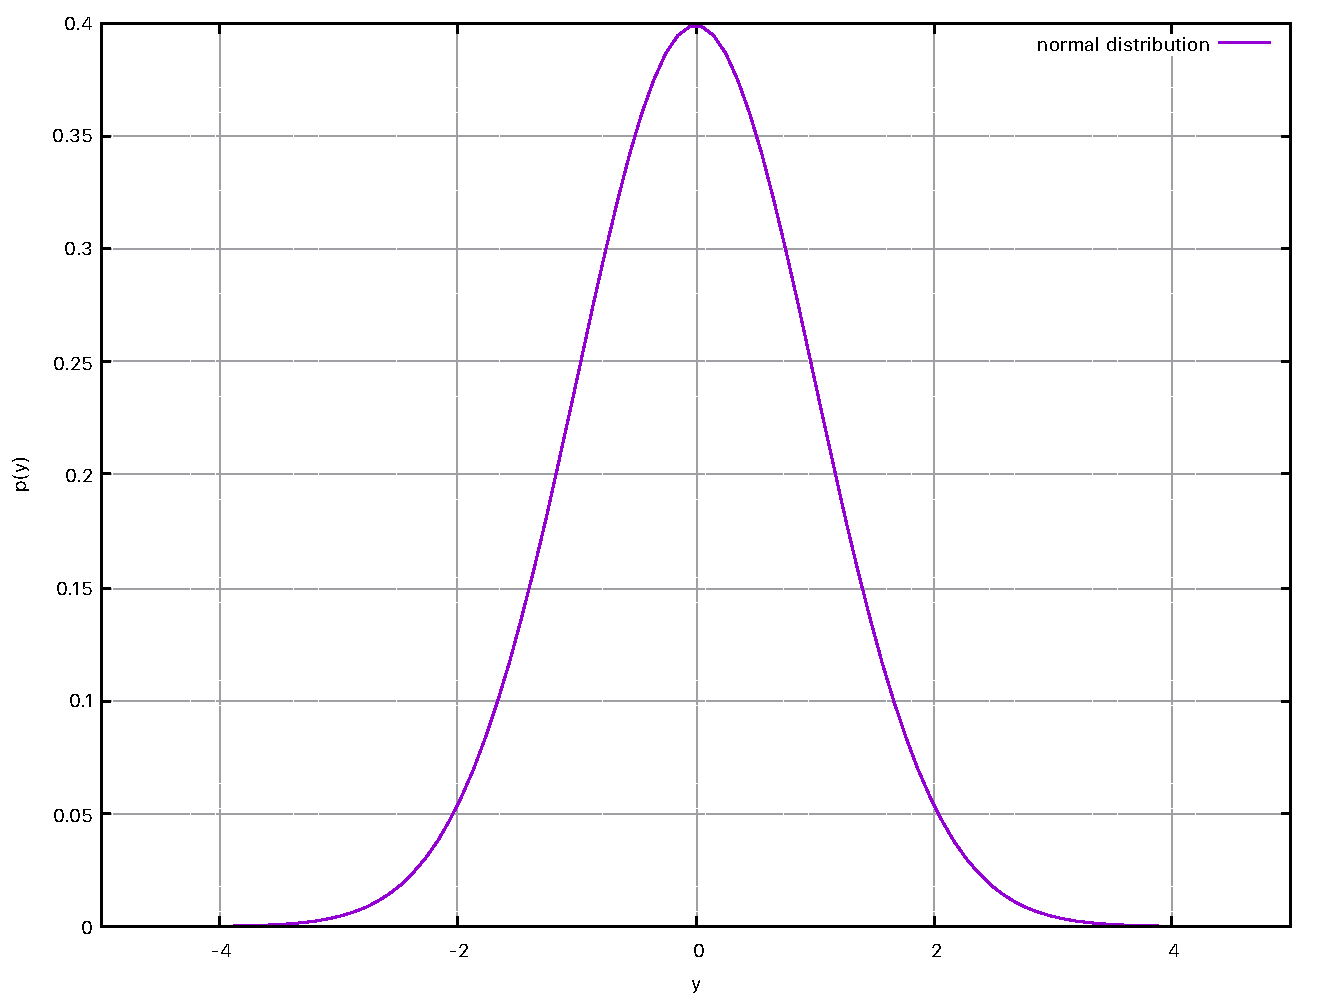
\includegraphics[scale=0.5]{/Users/ohyamasan/Downloads/TMCIT-Report/EE_Measurement/pre/plot.pdf}
\caption{正規分布}
\label{fig:normal-fig}
\end{figure}

\begin{equation}
\label{13}
p(x)=p(X=x)
\end{equation}

\begin{equation}
\label{eq:kakuritumitudo-fx}
p(x)=\frac{1}{\sqrt{2\pi}\sigma} \exp \left\{-\frac{(x-\mu)^2}{2\sigma^2}\right\}
\end{equation}

\begin{align}
\label{eq:int-nor}
\int_{-\infty}^{\infty} p(x)\,dx&=\frac{1}{\sqrt{2\pi}\sigma} \int_{-\infty}^{\infty} \exp \left(\frac{(x-\mu)^{2}}{2\sigma^{2}}\right)dx\nonumber\\
=&\frac{1}{\sqrt{2\pi}\sigma } \int_{-\infty}^{\infty} \exp \left(-\frac{y^{2}}{2\sigma^{2}}\right)dy\nonumber\\
=&\frac{1}{\sqrt{2\pi}\sigma }\sqrt{2\sigma^{2}\pi}=1
\end{align}

\subsubsection{平均値(mean)}
(算術)平均値とは$N$個全てのデータの総和を$N$個で割って得られる値で,\weq{heikinchi}で表すことができる\cite{1130848328216058496}.
\begin{equation}
	\bar{y} = \frac{1}{N}\sum^N_{i = 1}y_i
	\label{eq:heikinchi}
\end{equation}		

\subsubsection{標準偏差(standard deviation)\cite{1130000797042387712}}
標準偏差とは平均値を基準に各測定量がどれほどのばらついているかを定量的に表す値で,\weq{hyoujunhensa}で表すことができる.
\begin{equation}
	\sigma = \sqrt{\frac{1}{N - 1}\sum^N_{i = 1}(y_i - \bar{y})^2}
	\label{eq:hyoujunhensa}
\end{equation}	

\subsection{最小二乗法(method of least squares)\cite{1130848328216058496}\cite{1130282272174486912}}
2つの測定データ$y, x$間に一次方程式の関係があるとし,
\begin{equation}
	y = ax + b
	\label{eq:aiu}
\end{equation}
の傾き$a$,切片$b$を測定データからもっともらしい値にすることを考える.
その際に,
\begin{eqnarray}
	I &=& \sum\limits_{i=1}^{N} \varepsilon^2_i \nonumber\\
	&=& \sum\limits_{i=1}^{N} \bigl( y_i - f(x_i)\bigr)^2\nonumber\\\
	&=& \sum\limits_{i=1}^{N} \bigl( y_i - (ax_i+b)\bigr)^2
	\label{eq:error}
\end{eqnarray}
を最小にする$a$,$b$を求める.
これを最小二乗法といい,誤差を伴う測定値の処理においてその誤差の二乗の和を最小にすることで,最も確からしい関係式を求める方法である.前述の通り,誤差は正負あるため,2乘をしている.絶対値を用いると偏微分が不可能なため,平方根を用いた方法で行っている.
\begin{eqnarray}
	\frac{\partial}{\partial a}I(a,b) &=& 0\\
	\frac{\partial}{\partial b}I(a,b) &=& 0
\end{eqnarray}
から得られる方程式を,それぞれ$a$,$b$について解けば良く,それぞれの解を得るための方程式は次の2つを用いることになる.
\begin{equation}
	a = \frac{\sum_{n=1}^{n}(x_i -\bar{x})(y_i-\bar{y})}{\sum_{n=1}^{n}(x_i-\bar{x})^2}
	\label{eq:saisyou1}
\end{equation}
\begin{equation}
	b = \bar{y}-\frac{\sum_{n=1}^{n}(x_i -\bar{x})(y_i-\bar{y})}{\sum_{n=1}^{n}(x_i-\bar{x})^2} \bar{x}
	\label{eq:saisyou2}
\end{equation}
ここでは,\weq{aiu}のように1次式の形のものを示したが,一般に\weq{ippan}のような実験式に対して\weq{least-i}のように定義される.
\begin{align}
y&=F(x;a,b,c,\cdots)\label{eq:ippan}\\
(&xは変数,a,b,c,\cdots は定数)\nonumber
\end{align}
\begin{equation}
\label{eq:least-i}
I \equiv \sum_{i} (y_{i}-f(x_{i}))^{2} \quad \left(\frac{\partial I}{\partial a}=0 \to aを決定,\frac{\partial I}{\partial b}=0 \to bを決定 \cdots \right)
\end{equation}


\clearpage
\section{実験}
\subsection{ダイオードの特性実験}
\subsubsection{ダイオードの実験器具}
使用した実験器具を\wtab{kigu}に示す.
\begin{table}[h]
  \centering
  \caption{実験装置}
  \label{tab:kigu}
  \scalebox{1.0}{
  \begin{tabular}{cccccc}
    \hline
    機器名&製造元&型番&シリアル番号(または管理番号)\\
    \hline
    ダイオード&不明&1N4002&不明\\
    直流電源&YOKOGAWA&PA1811&L96-000668\\
    直流用電圧計&YOKOGAWA&YAS 1991&71 BA0 3371\\
    ミリアンペア直流用電流計&YOKOGAWA&YES 1990&70 BA0 1812\\
    マイクロアンペア直流用電流計&YOKOGAWA&B-5036.H1.10/10&B5036\\
    \hline
  \end{tabular}
}
\end{table}

\subsubsection{ダイオードの実験方法}
\begin{enumerate}[(1)]
	\item \wfig{bias}のように回路を構築した.なお,ダイオード$D$は1N4002を用いた.
	\item 順バイアス$E$を加え,電圧$V_{D}$(0から0.8\,\rm{V}まで0.1\,\rm{V}刻みで変化)と電流$I_{D}$を計測した.その際,電流計はミリアンペア計を利用し,端子は$300\,\rm{mA}$に接続した.
	\item 計測したデータをプロットし,データ数が不足していた$0.6\,\rm{V}$から$0.8\,\rm{V}$の区間は$V_{D}$を$0.025\,\rm{V}$刻みで計測した.
	\item 計測データを基に,$V_{D}-I_{D}$特性をグラフにまとめた.
	\item 回路を\wfig{bias}の回路でダイオード$D$を逆向きに接続するように変更し,逆バイアス$E$を$0\,\rm{V}$から$0.8\,\rm{V}$まで$1\,\rm{V}$刻みで加え,電流$V_{D}$と電流$I_{D}$を計測した.なお,電流はマイクロアンペア計で計測し,端子は$3\,\rm{mA}$に接続した.
	\item 順バイアスと同様に,$V_{D}-I_{D}$特性をグラフにまとめた.
	\begin{figure}[h]
	\centering
	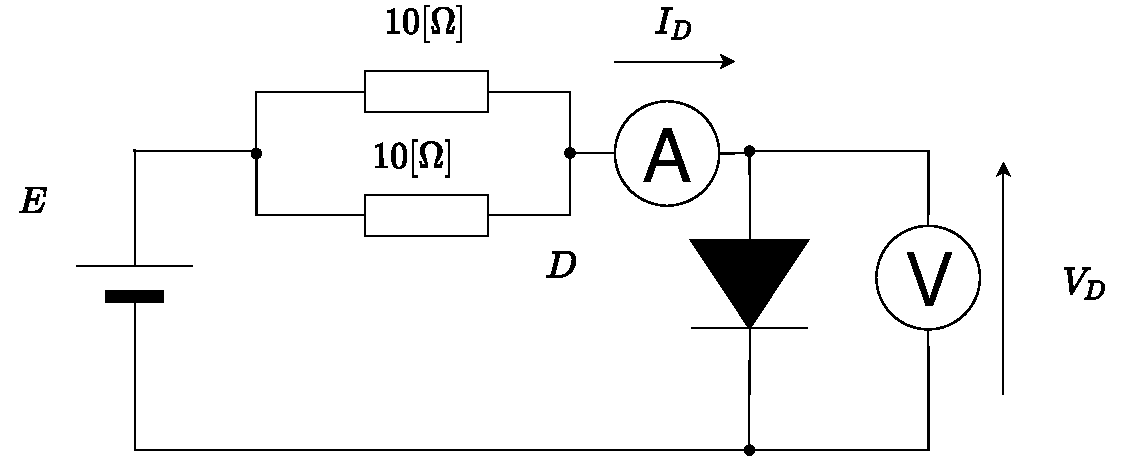
\includegraphics[scale=0.65]{./fig/bias.pdf}
	\caption{順バイアス測定回路}
	\label{fig:bias}
	\end{figure}
\end{enumerate}

\subsubsection{ダイオードの結果}
\begin{itemize}
	\item 測定結果を\wtab{bias}に示す.$0.400\,\rm{V}$まではほぼ電流が流れなかったが,それ以降は電圧増加とともに電流も増加し,$0.650\,\rm{V}$付近から急激に増加していることがわかる.
このような変化は抵抗の変化の仕方と異なっている.
	\item 順バイアスを印加した際の計測データから作成したグラフを近似曲線とともに\wfig{vias-graph-n}に示す.
	\item 逆バイアスを印加した際のグラフを\wfig{bias-rev}に示す.
	\begin{table}[h]
	\centering
	\caption{順・逆バイアスにおける電圧電流の関係}
	\label{tab:bias}
	\scalebox{1.0}{
	\begin{tabular}{cccc}
	\hline
	電圧(順バイアス)$V_{D}$[\rm{V}]  &電流$I_{D}$[\rm{mA}]   & 電圧(逆バイアス)$V_{D}$[\rm{V}] &  電流$I_{D}$[$\mu$\rm{A}] \\
	\hline
	0.000 & 0.0   & 0 & 0 \\
	0.100 & 0.0   & 1 & 0 \\
	0.200 & 0.0   & 2 & 0 \\
	0.300 & 0.0   & 3 & 0 \\
	0.400 & 0.0   & 4 & 0 \\
	0.500 & 1.0   & 5 & 0 \\
	0.600 & 2.0   & 6 & 0 \\
	0.625 & 4.0   & 7 & 0 \\
	0.650 & 6.0   & 8 & 0 \\
	0.675 & 10.0  &  - &  - \\
	0.700 & 19.8  &  - &  - \\
	0.725 & 29.0  & -  & -  \\
	0.750 & 48.0  & -  & -  \\
	0.775 & 71.0  & -  &  - \\
	0.800 & 116.0 & -  &-  \\
	\hline
	\end{tabular}
	}
\end{table}

\begin{figure}[h]
\centering
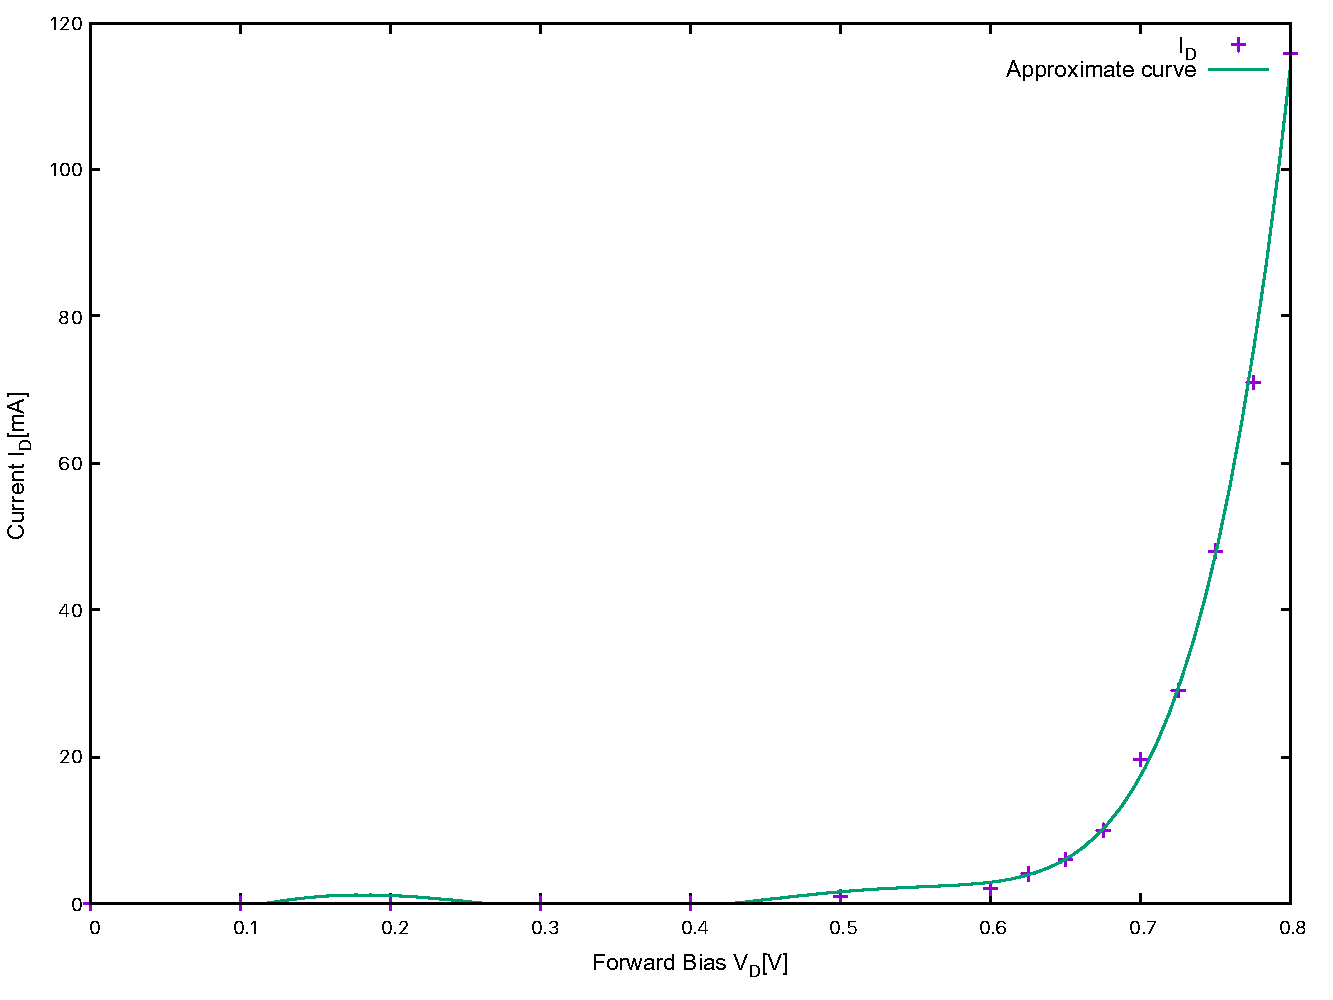
\includegraphics[scale=0.65]{./data/diode/bias-n.pdf}
\caption{順バイアスの$V_{D}-I_{D}$特性}
\label{fig:vias-graph-n}
\end{figure}
\end{itemize}

\begin{figure}[h]
\centering
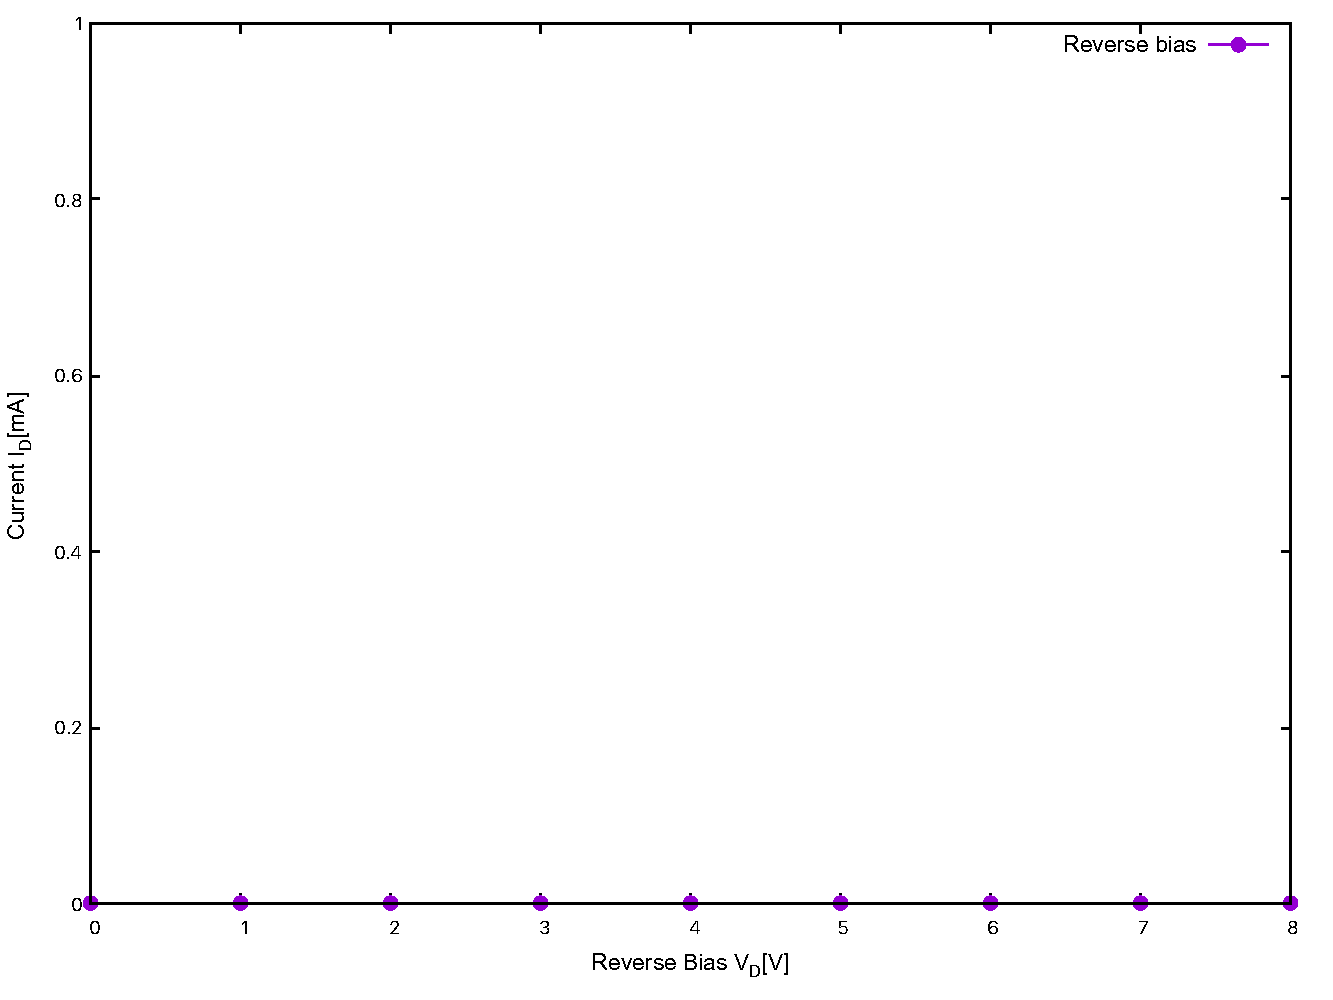
\includegraphics[scale=0.65]{./data/diode/bias-rev.pdf}
\caption{逆バイアスの$V_{D}-I_{D}$特性}
\label{fig:bias-rev}
\end{figure}

\clearpage
\subsubsection{ダイオードの考察}
\begin{enumerate}[(1)]
\item 直流電圧電流特性グラフを説明せよ.(立ち上がり電圧$V_{J}$をグラフに書き込む.また,$E=0.8\,\rm{V}$としたときの負荷線を描き,動作点Pの微分抵抗$r_{d}=\Delta V_{D}/\Delta I_{D}$を求めよ.$r_{d}$,$V_{J}$,理想ダイオードからなる等価回路を描き,どの部分がどのような特性を表しているのか説明せよ)

\wfig{vias-graph-n}に$V_{J}$,負荷線,を加えたグラフを\wfig{vias-graph-n-1}に示す.
また,各特性値の導出方法を\wtab{how}にまとめる.

\begin{table}[h]
\centering
\caption{特性値の導出方法}
\label{tab:how}
\scalebox{0.8}{
\begin{tabular}{cl}
\hline
特性値    & 導出方法  \\
\hline
動作点$P$ &負荷線の式(\weq{IF})に電圧$V_{D}$を代入した$I_{D}'$と計測電流$I_{D}$の誤差が最も少ない点($0.7\,\rm{V}$, $19.8\,\rm{mA}$)とした.(\wtab{PT}) \\
接線    & 動作点$P$を中間点とするような$(0.675\,\rm{V}, 10\,\rm{mA})$と$(0.725\,\rm{V}, 29\,\rm{mA})$を変位として\weq{int}のように導出 \\
$V_J$   & 接線と$x$軸との交点を通る$y$軸に並行な直線とした.(\weq{vj}) \\
負荷線   & \weq{IF}のように合成抵抗と電圧値により導出\cite{1130282271098203264}.\\
微分抵抗$r_d$ & 動作点$P$を中間点とするような$(0.675\,\rm{V}, 10\,\rm{mA})$と$(0.725\,\rm{V}, 29\,\rm{mA})$を変位として\weq{rd}のように算出\\
\hline
\end{tabular}
}
\end{table}

\begin{align}
\centering
I_{D}&=\frac{\Delta I_{D}}{\Delta V_{D}} V_{D} +V_{J}\nonumber \\
\frac{\Delta I_{D}}{\Delta V_{D}} &=\frac{(29-10)\times 10^{-3}}{0.725-0.675}=380\times 10^{-3}\,\rm{S}\nonumber \\
V_{J}&=I_{D}-\frac{\Delta I_{D}}{\Delta V_{D}} V_{D}\nonumber \\
この&接線は動作点を通るので\nonumber \\
&=19.8\times 10^{-3}-380\times 10^{-3}\cdot 0.7=-246.2\,\rm{mV}\nonumber \\
\therefore I_{D}&=380V_{D} -246.2[\rm{mA}]\label{eq:int}
\end{align}
\begin{align}
\centering
V_{J}の座標&は接線でI_{D}=0となる点であるから\weq{int}より\nonumber \\
0&=380V_{J} -246.2\nonumber \\
246.2&=380V_{J}\nonumber \\
\therefore V_{J}& \fallingdotseq 0.65\,\rm{V} \label{eq:vj}
\end{align}
\begin{align}
\centering
R&=\frac{10\cdot10}{10+10}\nonumber \\
&=5\,\rm{\Omega}\nonumber \\
I_{D}&=-\frac{1}{R}V_{D}+\frac{E}{R}\nonumber \\
&=-\frac{1}{5}V_{D}+\frac{0.8}{5}\,\rm{A}\nonumber \\
&=\left(-\frac{1}{5}V_{D}+\frac{0.8}{5}\right)\times 10^{3}[\rm{mA}]
\label{eq:IF}
\end{align}

\begin{table}[h]
\centering
\caption{動作点$P$の導出}
\label{tab:PT}
\scalebox{1.0}{
\begin{tabular}{cccc}
\hline
電圧$V_{D}$[\rm{V}]  &計測電流$I_{D}$[\rm{mA}]   & 算出した$I_{D}'$[\rm{mA}] & 誤差$|I_{D}-I_{D}'|$[\rm{mA}] \\
\hline
0.000 & 0.0   & 160 & 160 \\
0.100 & 0.0   & 140 & 140 \\
0.200 & 0.0   & 120 & 120 \\
0.300 & 0.0   & 100 & 100 \\
0.400 & 0.0   & 80  & 80  \\
0.500 & 1.0   & 60  & 59  \\
0.600 & 2.0   & 40  & 38  \\
0.625 & 4.0   & 35  & 31  \\
0.650 & 6.0   & 30  & 24  \\
0.675 & 10.0  & 25  & 15  \\
0.700 & 19.8  & 20  & 0.2 \\
0.725 & 29.0  & 15  & 14  \\
0.750 & 48.0  & 10  & 38  \\
0.775 & 71.0  & 5   & 66  \\
0.800 & 116.0 & 0   & 116 \\
\hline
\end{tabular}
}
\end{table}

\begin{figure}[h]
\centering
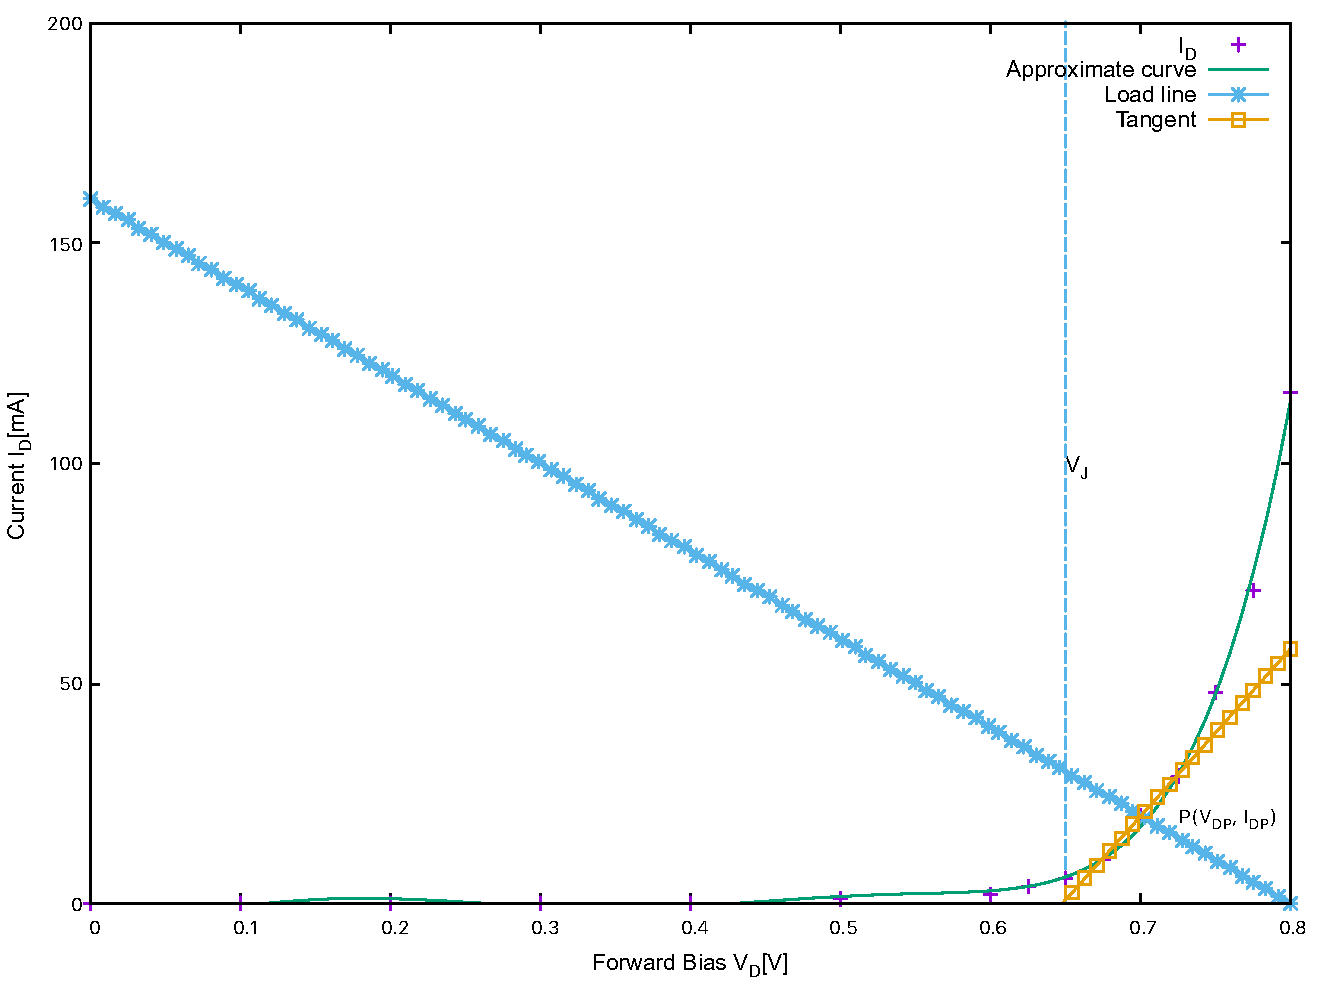
\includegraphics[scale=0.65]{./data/diode/bias-n-1.pdf}
\caption{順バイアスにおける負荷線と$V_{J}$}
\label{fig:vias-graph-n-1}
\end{figure}
\begin{align}
r_{d}&=\frac{\Delta V_{D}}{\Delta I_{D}}\nonumber \\
&=\frac{0.725-0.675}{(29.0-10.0)\times 10^{-3}}\nonumber \\
&=\frac{0.05}{19.0\times 10^{-3}}\nonumber \\
& \fallingdotseq 2.63\,\rm{\Omega}
\label{eq:rd}
\end{align}

理想ダイオードからなる等価回路は\wfig{eqc}となる~\cite{adsfcaw}.
$V_{J}$はダイオードの内部で発生する電界から生まれる電圧降下を示し,
$r_{d}$は動作点近傍でのダイオードの抵抗を表す~\cite{sdfvadfcdf}.
理想ダイオードは実際のダイオードと異なり,順方向にバイアスされているまたは,端子電圧が$0\,\rm{V}$の際に完全な導体として振る舞い,逆バイアスが印加されている時に完全な絶縁体となるものである.これらがダイオードの整流作用を起こしている~\cite{adsfcaw}.
	\begin{figure}[h]
	\centering
	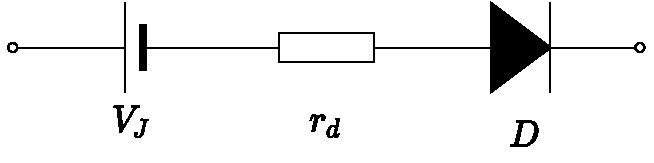
\includegraphics[scale=0.5]{./fig/eqc.pdf}
	\caption{理想ダイオードからなる等価回路}
	\label{fig:eqc}
	\end{figure}

	\item 実験で用いたダイオードのデータシートから逆方向電流の値を調べよ.また,逆バイアスの場合でもわずかに電流が流れる理由を図を用いて説明せよ.(多数キャリアや少数キャリアという観点から考えること。\wfig{fig2}を用いるとよい.)

データシート~\cite{sdfgvhsd}より逆電流$I_{R}$は$25^{\circ}$Cで最大$10\,\rm{\mu A}$流れることがわかる.
逆バイアスを印加した際,接合面で多数キャリアが再結合で減少する.
また\wfig{fig2}ではp型において,多数キャリアのみに注目しているため,電子が移動せず,電流が流れないように考えられるが,実際は少数キャリアである電子が移動する(ドリフト)ためわずかに電流が流れてしまう.
\end{enumerate}

\clearpage
\subsection{ツェナーダイオードの特性実験}
\subsubsection{ツェナーダイオードの実験器具}
使用した実験器具を\wtab{kigu2}に示す.
\begin{table}[h]
  \centering
  \caption{実験装置}
  \label{tab:kigu2}
  \scalebox{1.0}{
  \begin{tabular}{cccccc}
    \hline
    機器名&製造元&型番&シリアル番号(または管理番号)\\
    \hline
    ダイオード&不明&1N4736A&不明\\
    直流電源&YOKOGAWA&PA1811&L96-000668\\
    直流用電圧計&YOKOGAWA&YAS 1991&71 BA0 3371\\
    ミリアンペア直流用電流計&YOKOGAWA&YES 1990&70 BA0 1812\\
    \hline
  \end{tabular}
}
\end{table}

\subsubsection{ツェナーダイオードの実験方法}
\begin{enumerate}[(1)]
\item \wfig{zenerc}のように回路を構築する.なお,電圧計は$10\,\rm{V}$端子,電流計は$30\,\rm{mA}$端子に接続して計測を行った.また,配線時にダイオードの向きに注意する必要がある.
\item $V_{i}$を$0\,\rm{V}$から$18\,\rm{V}$まで$0.1\,\rm{V}$刻みで増加させ,電流$I_{Z}$と電圧$V_{L}$を計測する.
\item 上記で計測したデータをもとに,$V_{i}-V_{L}$特性,$V_{i}-I_{Z}$を同一グラフに描画した.
\begin{figure}[h]
\centering
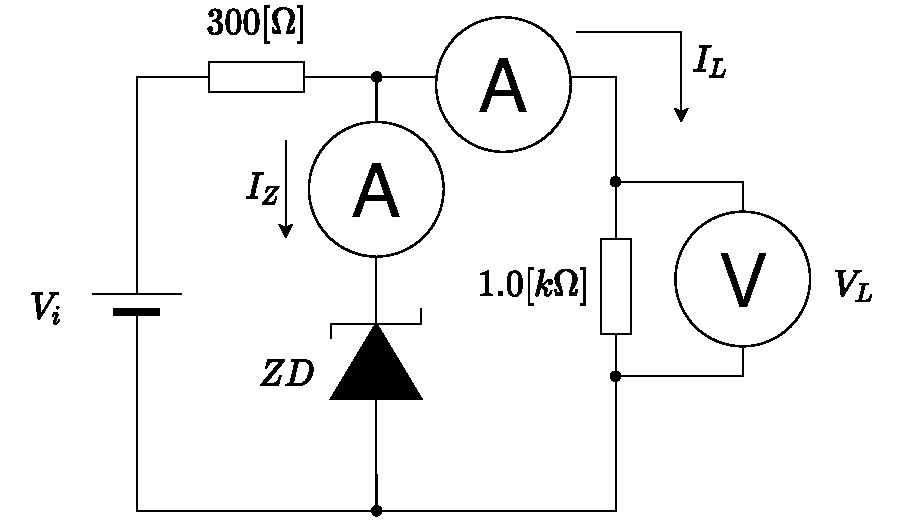
\includegraphics[scale=0.7]{./fig/zenerc.pdf}
\caption{ツェナーダイオード測定回路}
\label{fig:zenerc}
\end{figure}
\end{enumerate}

\subsubsection{ツェナーダイオードの結果}
\begin{itemize}
\item \wtab{zener-tab}に測定したデータをまとめた.
出力電圧が$10\,\rm{V}$付近からツェナー電流の増加が起きていることがわかる.
また,出力電圧$V_{L}$は$8\,\rm{V}$以降,入力電圧が増加してもあまり変化が起きていない.
\item \wfig{zenerg}は$V_{i}-V_{L}$特性,$V_{i}-I_{Z}$特性のグラフである.$V_{L}$は増加した後,ほぼ一定となっているのに対し,$I_{Z}$はほぼ一定($=0$)の後,増加と逆の動きをしている.
\begin{table}[h]
\centering
\caption{ツェナーダイオードの特性}
\label{tab:zener-tab}
\scalebox{0.9}{
\begin{tabular}{ccc}
\hline
入力電圧$V_i$$[\rm{V}]$ & 出力電圧$V_L$$[\rm{V}]$ & ツェナー電流$I_Z$$[\rm{mA}]$ \\
\hline
0    & 0.0       & 0.0      \\
1    & 0.8     & 0.0       \\
2    & 1.5       & 0.0          \\
3    & 2.3         & 0.0              \\
4    & 3.0           & 0.0              \\
5    & 3.8         & 0.0              \\
6    & 4.6         & 0.0           \\
7    & 5.3         & 0.0              \\
8    & 6.1         & 0.0           \\
9    & 6.8         & 0.1       \\
10   & 6.9         & 3.0           \\
11   & 6.9         & 6.2          \\
12   & 7.0           & 9.6           \\
13   & 7.0           & 12.8           \\
14   & 7.0           & 16.1           \\
15   & 7.0           & 19.4           \\
16   & 7.1         & 22.6        \\
17   & 7.1         & 25.9           \\
18   & 7.2      & 29.2     \\
\hline
\end{tabular}
}
\end{table}
\begin{figure}[h]
\centering
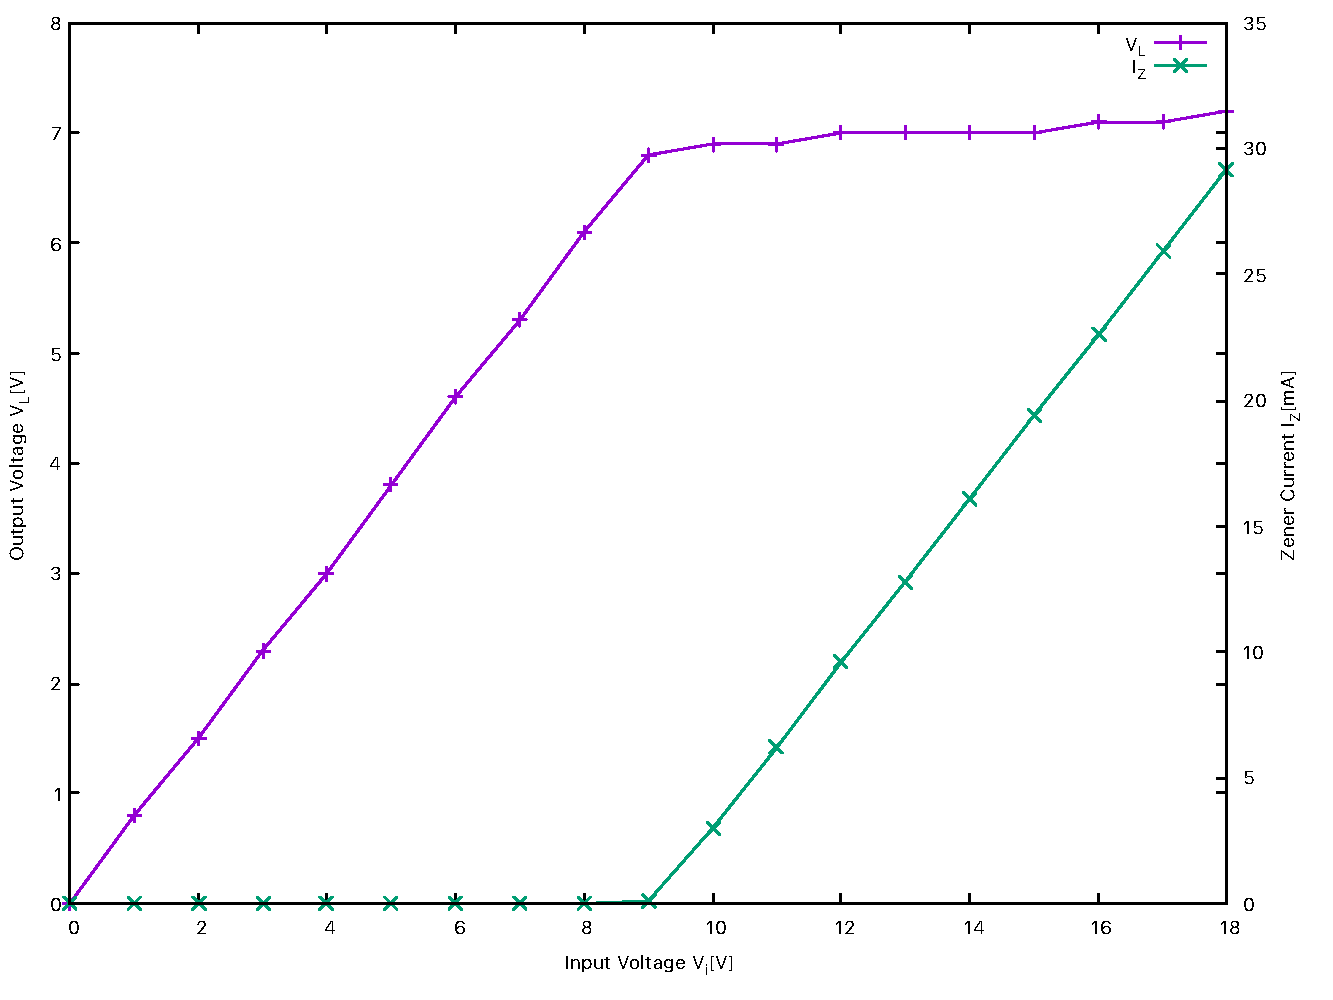
\includegraphics[scale=0.65]{./data/zener/zener-graph.pdf}
\caption{ツェナーダイオードの特性}
\label{fig:zenerg}
\end{figure}
\end{itemize}

\clearpage
\subsubsection{ツェナーダイオードの考察}
\begin{enumerate}[(1)]
\item 今回用いたツェナーダイオード1N4736Aをダイオード規格表(または,データシート)でツェナー電圧を調べ,実験結果と比較して考察せよ.

データシート~\cite{fbklsdn}を参照すると平均値は$6.8\,\rm{V}$($25^{\circ}$C)である.一方,実験結果より,ツェナー電圧は$6.8\,\rm{V}$から$7.2\,\rm{V}$で推移しており,データシートとの差異がほとんどなく,正しく計測できたといえる.
\item ツェナーダイオードはどういった場合に用いられるか説明せよ.

ツェナーダイオードは\wfig{diode-vi-curve-03}からわかるように,逆電圧を一定(降伏電圧, $V_{R}$)以上かけると急激に電流が流れるようになる特性がある.
この降伏電圧付近では,電流の広い範囲にわたって電圧が一定である.
すなわち,ダイオードに流れる電流の大きさに依存せずダイオードの電圧は一定に保たれるため.定電圧源として利用される\cite{1130282271098203vsdv4}.
\begin{figure}[h]
\centering
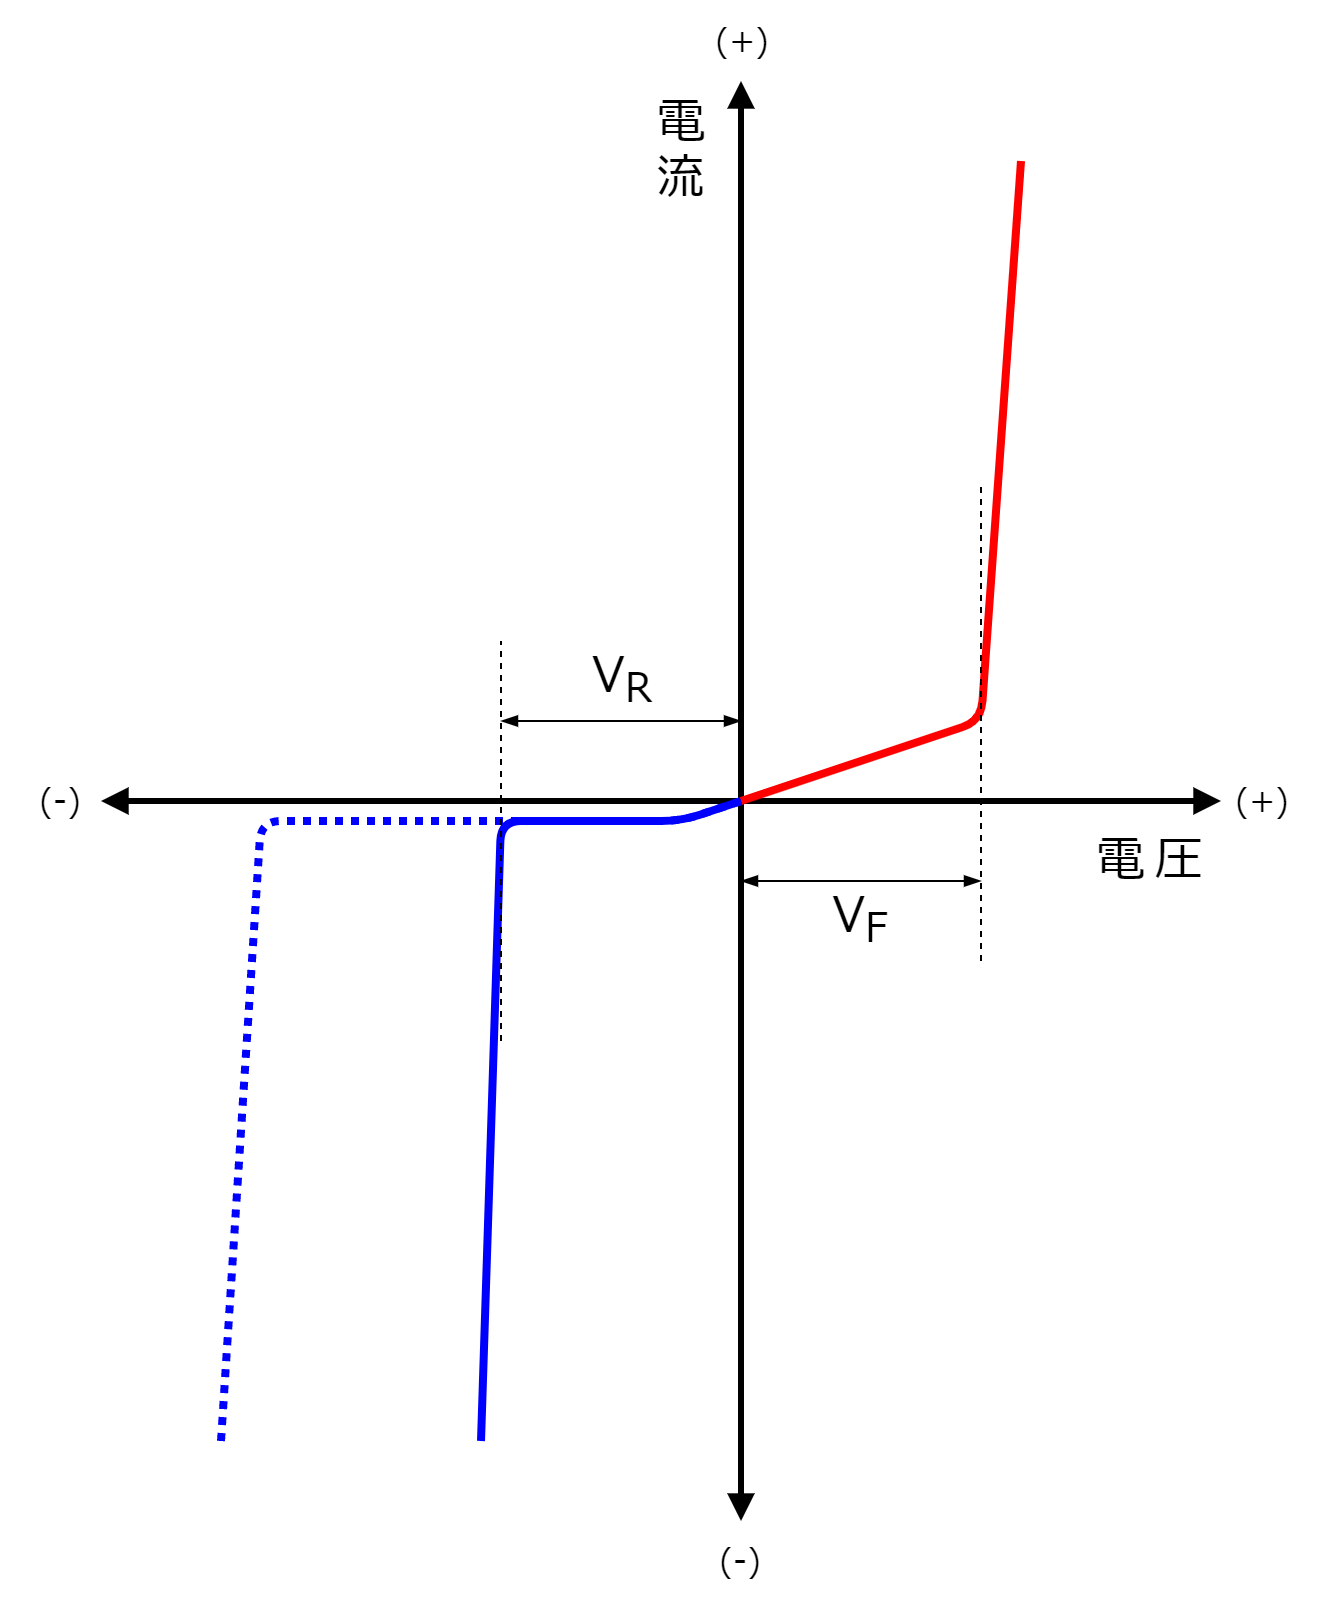
\includegraphics[scale=0.15]{./fig/diode-vi-curve-03.png}
\caption{ツェナーダイオードの特性図\cite{sdjabcklds}}
\label{fig:diode-vi-curve-03}
\end{figure}
\item  $V_{Z}-I_{Z}$特性のグラフを描き,ツェナー電圧$V_{Z}$を明記せよ.

\wfig{zener-v-i}に$V_{Z}-I_{Z}$特性を示す.なお,$V_{Z}$は$6.8\,\rm{V}$とした.
出力電圧はほぼツェナー電圧に近似できているが,実験結果と誤差が少し発生している.
\begin{figure}[h]
\centering
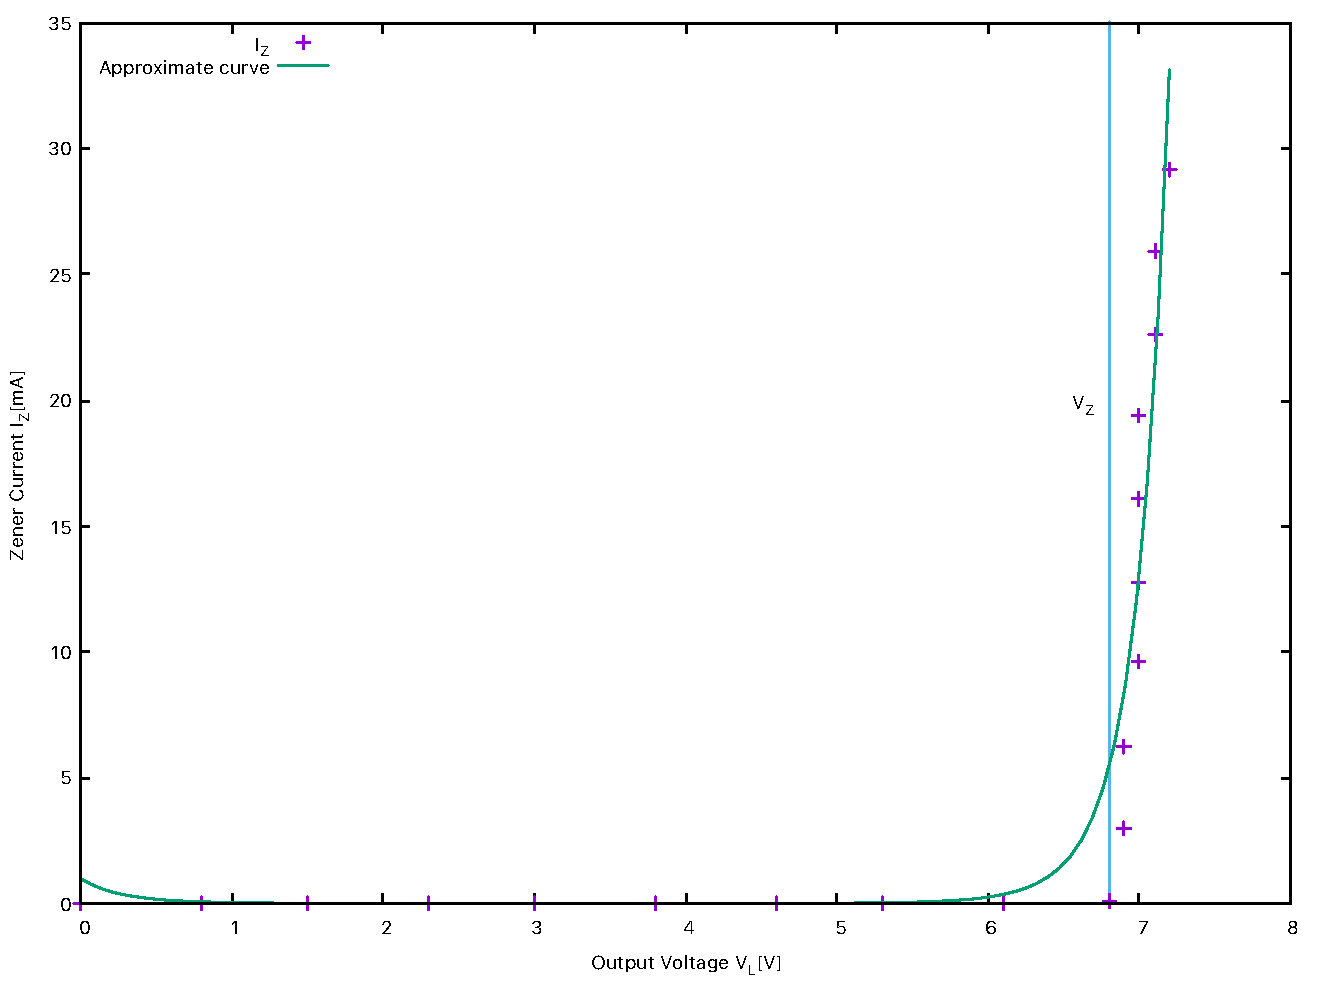
\includegraphics[scale=0.7]{./data/zener/zener-v-i.pdf}
\caption{ツェナーダイオードの特性}
\label{fig:zener-v-i}
\end{figure}
\item 各グラフから入出力特性を考察せよ.

入力特性($V_{i}-I_{Z}$)について考える.\\
\wfig{zenerg}より,立ち上がり電圧$V_{F}$は$0.9\,\rm{V}$で,以降$I_{Z}$は$V_{i}$とほぼ比例して増加している.その傾きは約$33\times 10^{-3}\,\rm{S}$である.\\
次に出力特性($V_{L}-I_{Z}$)について考える.\\
\wfig{zener-v-i}より,$V_{Z}$以降,急激に電流を通すようになる.そしてその時の電圧は$6.8\,\rm{V}$から$7.3\,\rm{V}$に落ちついている.
\end{enumerate}

\clearpage
\subsection{ツェナーダイオード定電圧回路の実験}
\subsubsection{ツェナーダイオード定電圧回路の実験器具}
使用した実験器具を\wtab{kigu3}に示す.
\begin{table}[h]
  \centering
  \caption{実験装置}
  \label{tab:kigu3}
  \scalebox{0.9}{
  \begin{tabular}{cccccc}
	\hline
	機器名&製造元&型番&シリアル番号(または管理番号)\\
	\hline
	ダイオード&不明&1N4736A&不明\\
	直流電源&YOKOGAWA&PA1811&L96-000668\\
	直流用電圧計&YOKOGAWA&YAS 1991&71 BA0 3371\\
	ミリアンペア直流用電流計&YOKOGAWA&YES 1990&70 BA0 1812\\
	可変抵抗器&TOKUSHU DENKI KOGYOSHO&S-3&3201\\
	\hline
  \end{tabular}
}
\end{table}

\subsubsection{ツェナーダイオード定電圧回路の実験方法}
\begin{enumerate}[(1)]
	\item \wfig{zenerc-2}のように回路を構築する.なお,ダイオード$ZD$は1N4736Aを使用した.
\begin{figure}[h]
	\centering
	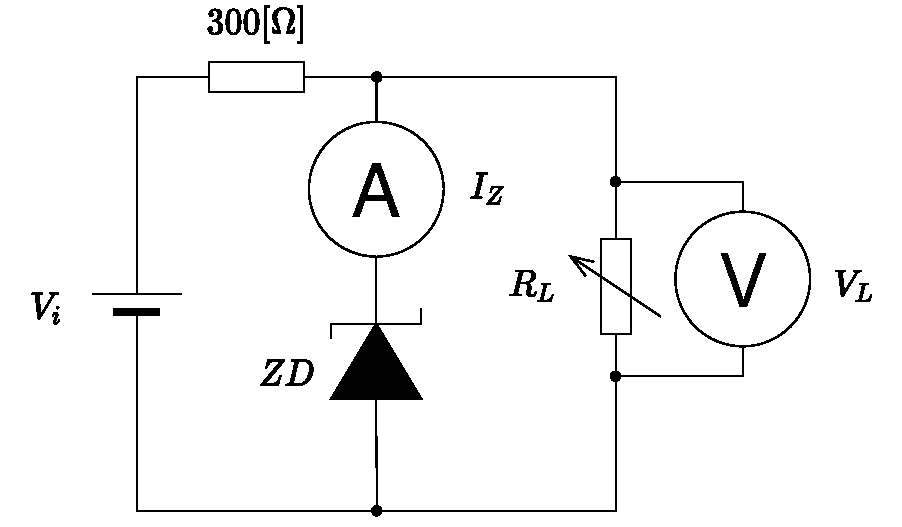
\includegraphics[scale=0.65]{./fig/zenerc-2.pdf}
	\caption{ツェナーダイオード定電圧測定回路}
	\label{fig:zenerc-2}
\end{figure}
	\item 入力$V_i$を$15\,\rm{V}$に固定し,可変抵抗$R_{L}$を変化させてツェナー電流$I_Z$を$2\,\rm{mA}$刻みで$2\,\rm{mA}$から$22\,\rm{mA}$まで変化させた.その際,電流計は端子$30\,\rm{mA}$に接続した.
	\item それぞれの場合で,出力電圧$V_L$と,出力電流$I_Z$を計測した.
	\item 上記のデータを元に$I_{Z}-V_{Z}$,$I_Z-I_L$のグラフを作成した.
\end{enumerate}

\subsubsection{ツェナーダイオード定電圧回路の結果}
\begin{itemize}
	\item \wfig{zener-const-1}に$I_{Z}-V_{Z}$,\wfig{zener-const-2}に$I_{Z}-I_{L}$特性グラフを示す.
出力電圧$V_L$はツェナー電流$I_Z$に依存せず,$7\,\rm{V}$付近で一定であった.
また,出力電流$I_{L}$はツェナー電流$I_Z$増加とともにほぼ比例的に減少している.
\begin{figure}[h]
	\centering
	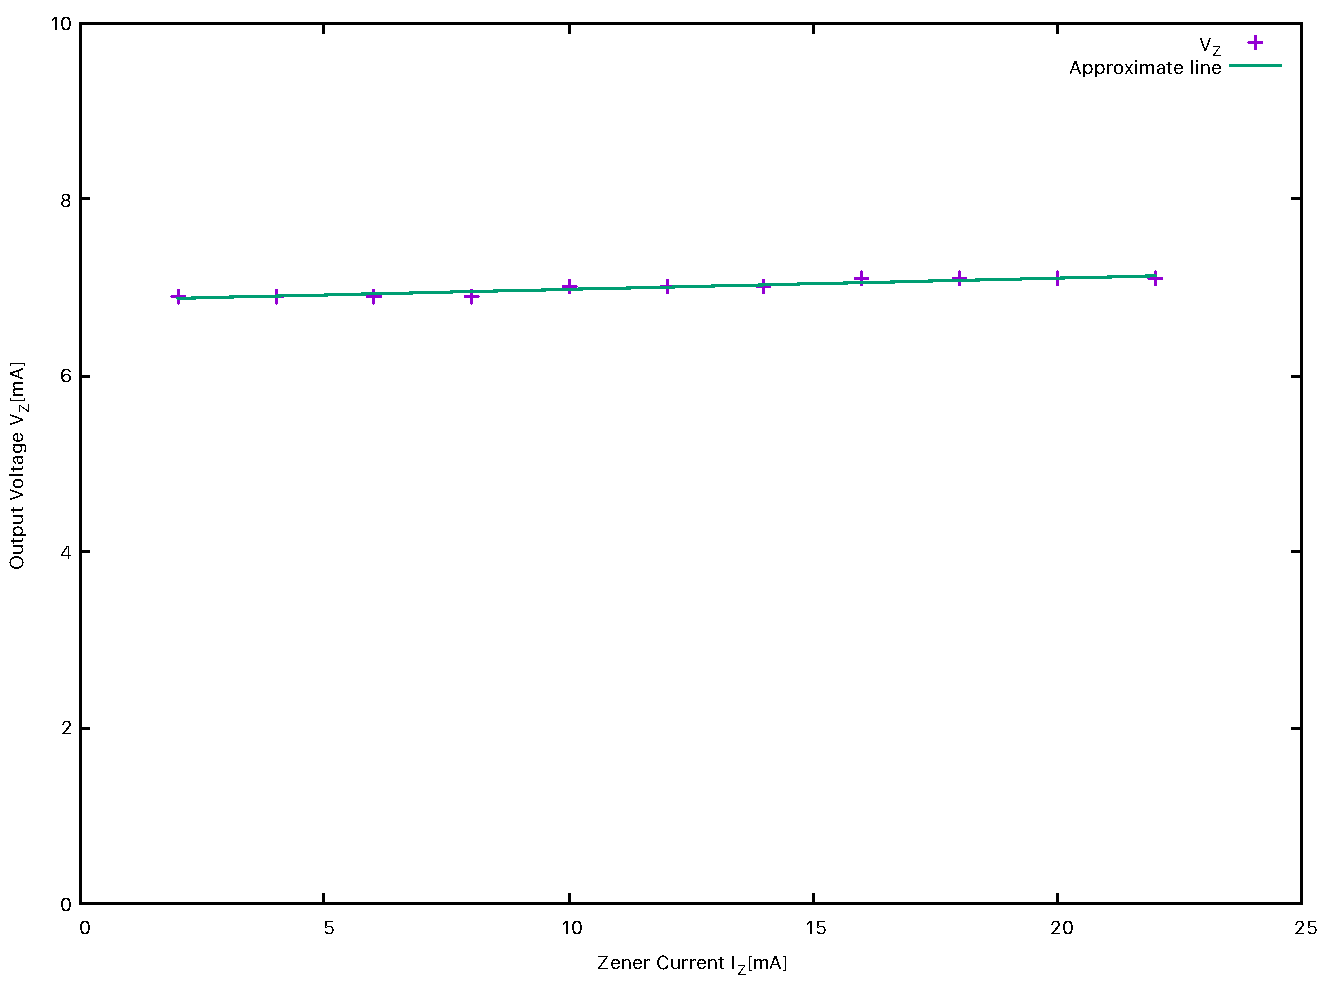
\includegraphics[scale=0.65]{./data/zener/zener-const-1.pdf}
	\caption{定電圧回路の$I_Z-V_Z$特性}
	\label{fig:zener-const-1}
\end{figure}
\begin{figure}[h]
	\centering
	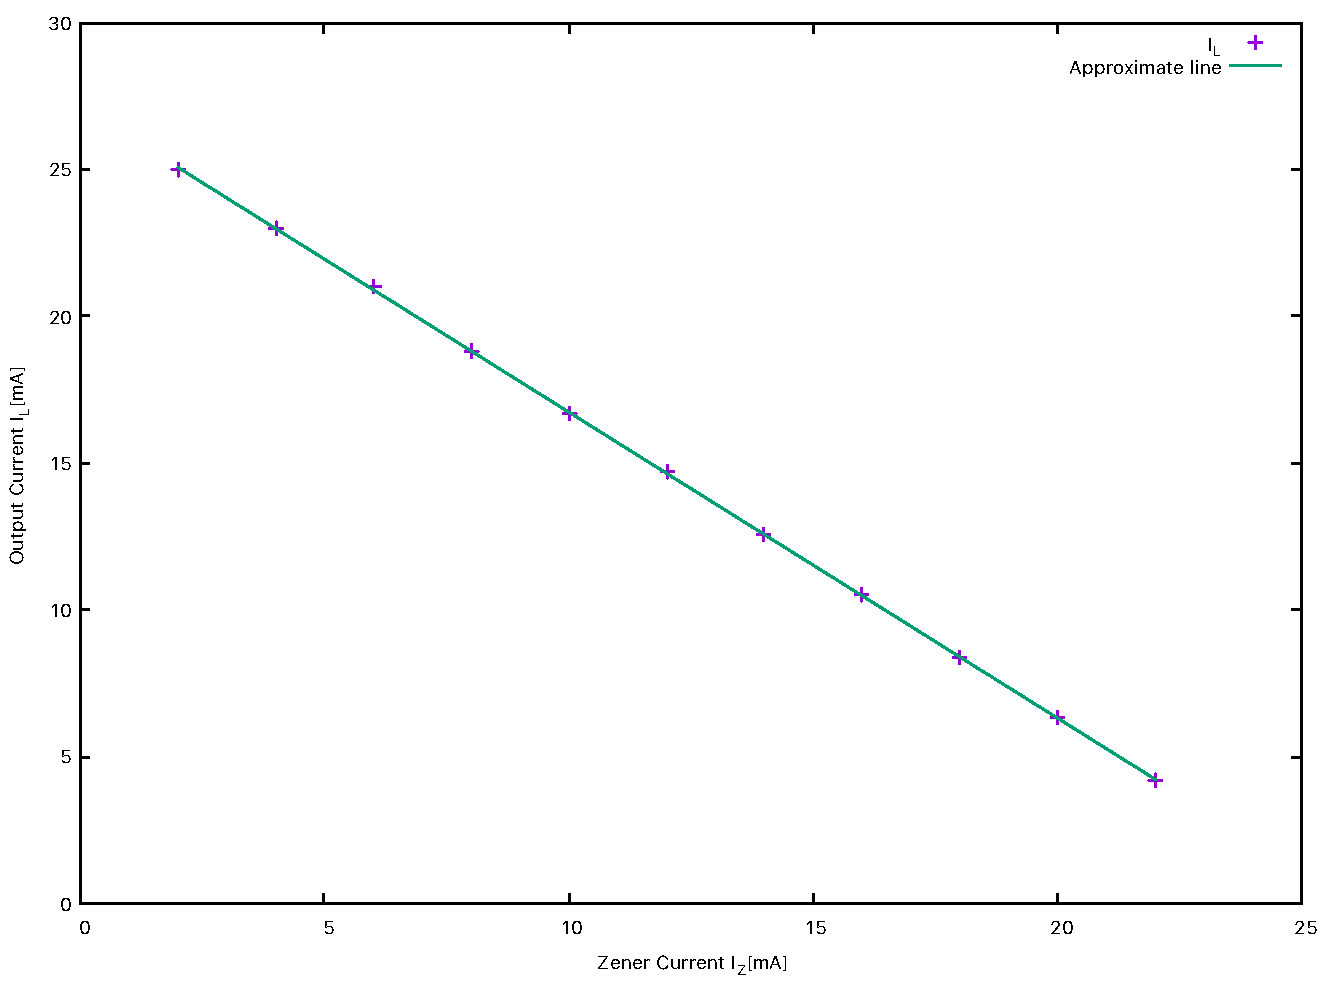
\includegraphics[scale=0.65]{./data/zener/zener-const-2.pdf}
	\caption{定電圧回路の$I_Z-I_L$特性}
	\label{fig:zener-const-2}
\end{figure}
\end{itemize}

\clearpage
\subsubsection{ツェナーダイオード定電圧回路の考察}
\begin{enumerate}[(1)]
	\item 等価回路図(\wfig{zener-eq})を参考にして,測定結果から$R_{L}$,$R_{Z}$,およびこれらの合成抵抗$R_{A}$を算出せよ.
	
	\begin{figure}[h]
	\centering
	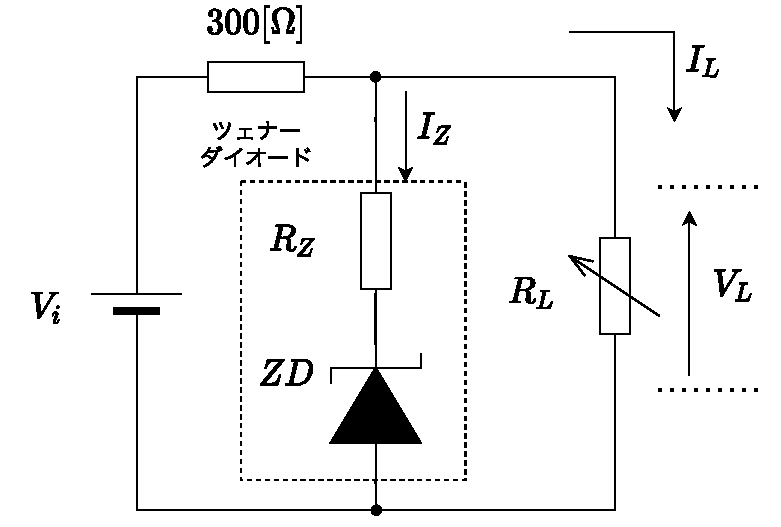
\includegraphics[scale=0.75]{./fig/zener-eq.pdf}
	\caption{ツェナーダイオード定電圧等価回路}
	\label{fig:zener-eq}
	\end{figure}
	\wfig{zener-eq}より,この回路は並列回路であることがわかり,分圧則とオーム則を用いて抵抗値が算出可能である.
	\weq{RL}から\weq{RA}に各抵抗値の導出方法を示す.
\begin{align}
	R_{L}&=\frac{V_{L}}{I_{L}}\label{eq:RL}\\
	R_{Z}&=\frac{V_{L}}{I_{Z}}\label{eq:RZ}\\
	R_{A}&=300+\frac{R_{Z}\cdot 1.0\times 10^{3}}{R_{Z}+1.0\times 10^{3}}\label{eq:RA}
\end{align}
	これらの計算を各ツェナー電流ごとに行ったものを\wtab{rtab}に示す.
	
\begin{table}[h]
\centering
\caption{電流,電圧値により算出した各抵抗値}
\label{tab:rtab}
\scalebox{1.0}{
\begin{tabular}{cccc}
	\hline
	ツェナー電流$I_{Z}$[$\rm{mA}$] & 可変抵抗値$R_{L}$[$\Omega$] & ダイオード抵抗値$R_{Z}$[$\Omega$] & 合成抵抗$R_{A}$[$\Omega$]  \\
	\hline
	 2     & 0.276 & 3.450    & 0.256 \\
	 4     & 0.300 & 1.725    & 0.256 \\
	 6     & 0.329 & 1.150    & 0.256 \\
	 8     & 0.367 & 0.863    & 0.257 \\
	10    & 0.419 & 0.700    & 0.262 \\
	12    & 0.476 & 0.583    & 0.262 \\
	14    & 0.556 & 0.500    & 0.263 \\
	16    & 0.676 & 0.444    & 0.268 \\
	18    & 0.845 & 0.394    & 0.269 \\
	20    & 1.127 & 0.355    & 0.270 \\
	22    & 1.690 & 0.323    & 0.271 \\
	\hline
\end{tabular}
}
\end{table}
この表より,合成抵抗$R_{A}$はほとんどツェナー電流に依存せずに一定の値をとっていることがわかる.このことは,\weq{ZL}で右辺の項が定数のため,左辺の電流値も定数となっているためである.
\begin{equation}
	I_{Z}+I_{L}=\frac{V_{i}-V_{L}}{300}
	\label{eq:ZL}
\end{equation}
\begin{figure}[h]
	\centering
	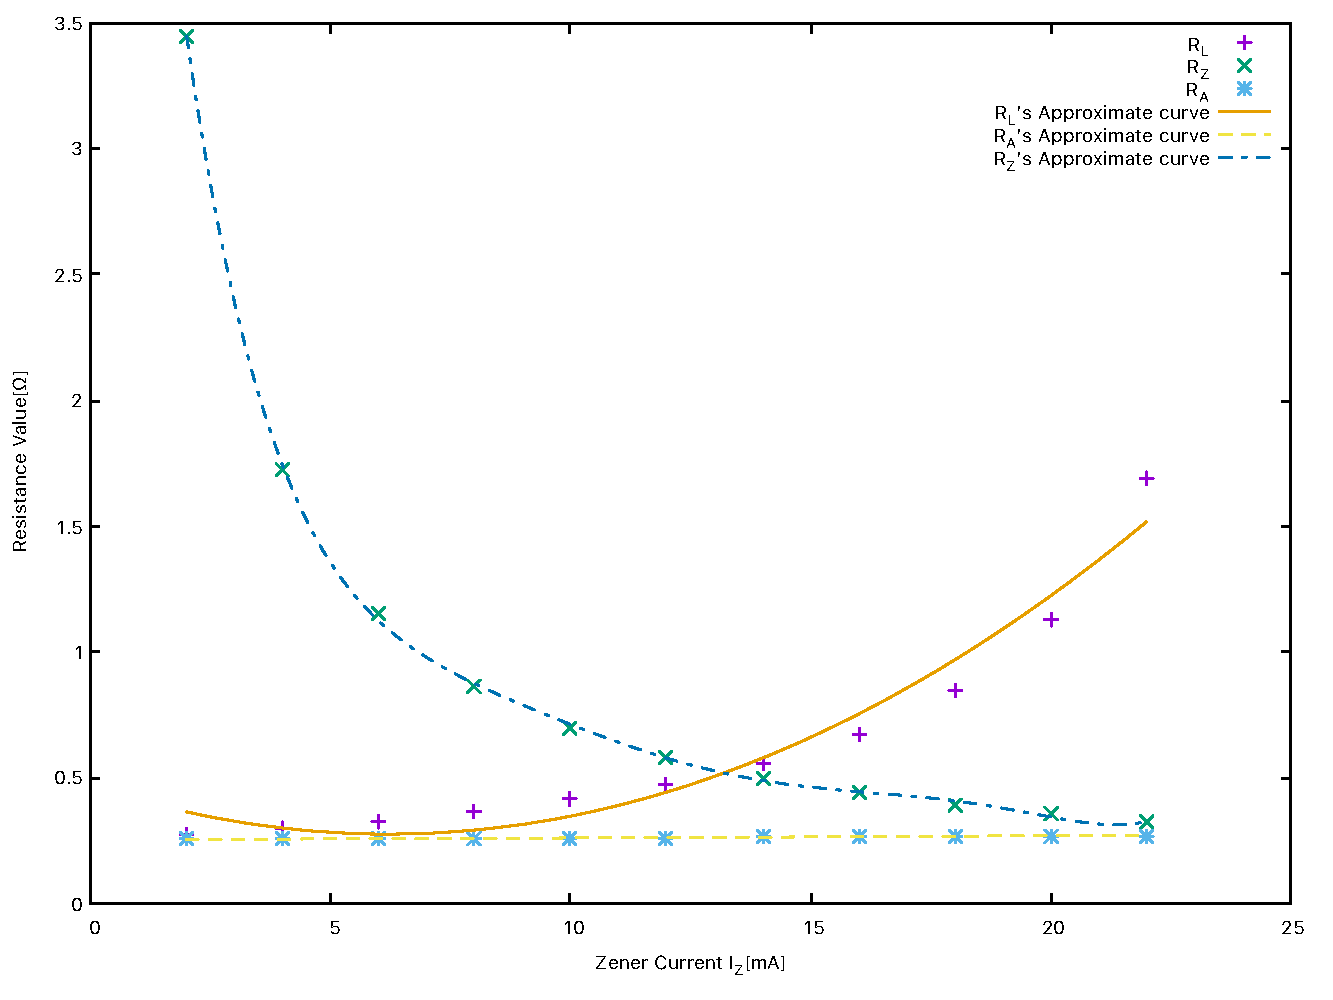
\includegraphics[scale=0.7]{./data/zener/r.pdf}
	\caption{各抵抗のツェナー電流特性}
	\label{fig:rgraph}
\end{figure}
	\item $I_{Z}-R_{L}$特性,$I_{Z}-R_{Z}$特性を同一グラフに重ねて描き,考察せよ.ここで,何について論じたいかを明確にした上で記述すること.

	\wfig{rgraph}は上記式により導出した各抵抗値のツェナー電流特性である.
	合成抵抗はツェナー電流の変化に依存していないが,$R_{L}$は$I_{Z}$に比例し,$R_{Z}$は反比例していることが読み取れる.これは上の考察と矛盾がない.
\end{enumerate}
\clearpage
\subsection{太陽電池の発電特性の実験}

\subsubsection{太陽電池の発電特性の実験器具}
使用した実験器具を\wtab{kigu4}に示す.
\begin{table}[h]
  \centering
  \caption{実験装置}
  \label{tab:kigu4}
  \scalebox{0.7}{
  \begin{tabular}{cccccc}
	\hline
	機器名&製造元&型番&シリアル番号(または管理番号)\\
	\hline
	太陽電池&SUNYO&SY-M5W&-\\
	ディジタル照度計& Zhangzhou Weihua Electronic Co., Ltd&LX-1010B&T 428585\\
	ディジタル温度計&Gain Express Holdings&THE-27 Digital Thermometer 4 Channel K-Type&202019031\\
	ディジタルマルチメータ&owon&B35&B351518443\\
	可変抵抗器&TOKUSHU DENKI KOGYOSHO&S-3&3201\\
	\hline
  \end{tabular}
}
\end{table}

\subsubsection{太陽電池の発電特性の実験方法}
\begin{enumerate}[(1)]
	\item \wfig{solar-cell}のように回路を構築する.
	\begin{figure}[h]
	\centering
	\includegraphics[scale=0.5]{./fig/solar-cell.pdf}
	\caption{太陽電池の計測回路}
	\label{fig:solar-cell}
	\end{figure}
	\item 太陽電池はライトの光が均等に照射されるように配置した.
	\item 可変抵抗器のレバーを短絡側にセットし,ライトを2つ点灯させた.
	\item 太陽電池を動かし,電流が最大になる位置を探し位置に印をつけた.
	\item ライトを1つ点灯に変更した.
	\item 太陽電池の四隅と中央の計5ヶ所に関して計測を行い.その平均値を代表値として,算出した.
	\item 太陽電池の裏面中央に温度計を設置した.
	\item 照度測定後,太陽電池温度が$30^{\circ}$Cになるように調節を行った.\label{ondo}
	\item $V-I$測定を開始した.可変抵抗$R_{L}$を変更させながら,電流$I$,電圧$V$を記録する.$V_{oc}$付近ではデータ取得間隔を細かくした.\label{I-V}
	\item 測定の際温度は$\pm 2^\circ$Cの範囲で計測を行った.
	\item 点灯させるライトを2つに変更し,上記と同様((\ref{ondo}) $\sim$ (\ref{I-V}))に計測を行った.
	\item 太陽電池温度を$50^{\circ}$Cに変更し,点灯させるライトを1つ,2つの場合に対し測定を行った.
\end{enumerate}

\subsubsection{太陽電池の発電特性の結果}
\label{solar-cell-result}
\begin{itemize}
	\item $30^{\circ}$C,ライト1つ・2つ,$50^{\circ}$C,ライト1つ・2つの計4条件での計測結果を\wtab{30-one}$\sim$\wtab{50-two}に示す.
	上記データをもとに作成した,$V-I$カーブを\wfig{VIc}に示す.
	
	これらより電流が多く流れることに関わる因子の影響は,太陽電池温度ではなく,ライトの個数(照度)の方が大きいことがわかる.また,出力される電流の最大値は決まっており,ある電圧を超えるとほぼ一定であった電流値が減少に変化することが確認される.
	そして,その電圧の値は4条件で大きく違いがなかった.
	\item \weq{power}をExcelを用いて算出した電力を用いて作成した$V-P$カーブを\wfig{VPc}に示す.
	\begin{equation}
		P=VI
		\label{eq:power}
	\end{equation}
	\begin{table}[p]
	\begin{tabular}{cc}
	\begin{minipage}[t]{0.5\hsize}
	\centering
	\caption{$30^{\circ}$C ライト1つの場合(照度8600\,\rm{lux})}
	\label{tab:30-one}
	\scalebox{1.0}{
	\begin{tabular}{ccc}
	\hline
	電圧$V$[\rm{V}] & 電流$I$[\rm{mA}]   & 電力$P$[\rm{W}] \\
	\hline
	0.8  & 63.8 & 0.1 \\
	2.8  & 63.7 & 0.2 \\
	3.5  & 63.0 & 0.2 \\
	7.0  & 63.1 & 0.4 \\
	9.8  & 62.6 & 0.6 \\
	12.3 & 62.3 & 0.8 \\
	14.3 & 61.9 & 0.9 \\
	16.7 & 61.5 & 1.0 \\
	17.3 & 60.0 & 1.0 \\
	18.3 & 56.5 & 1.0 \\
	18.7 & 50.2 & 0.9 \\
	18.9 & 45.3 & 0.9 \\
	19.2 & 40.5 & 0.8 \\
	19.4 & 35.3 & 0.7 \\
	19.5 & 30.7 & 0.6 \\
	19.6 & 25.7 & 0.5 \\
	20.0 & 20.5 & 0.4 \\
	20.1 & 15.5 & 0.3 \\
	20.1 & 10.6 & 0.2 \\
	20.2 & 6.1  & 0.1 \\
	\hline
	\end{tabular}
	}
	\end{minipage}
	\begin{minipage}[t]{0.5\hsize}
	\centering
	\caption{$30^{\circ}$C ライト2つの場合}
	\label{tab:30-two}
	\scalebox{0.9}{
	\begin{tabular}{ccc}
	\hline
	電圧$V$[\rm{V}]   & 電流$I$[\rm{mA}]   & 電力$P$[\rm{W}]  \\
	\hline
	1.9  & 151.1 & 0.3 \\
	2.7  & 151.0 & 0.4 \\
	3.9  & 148.8 & 0.6 \\
	5.6  & 148.3 & 0.8 \\
	7.1  & 147.2 & 1.0 \\
	9.9  & 144.0 & 1.4 \\
	10.7 & 141.5 & 1.5 \\
	15.9 & 137.6 & 2.2 \\
	13.7 & 141.0 & 1.9 \\
	18.6 & 136.4 & 2.5 \\
	19.3 & 127.5 & 2.5 \\
	19.7 & 105.8 & 2.1 \\
	20.0 & 91.2  & 1.8 \\
	20.4 & 80.3  & 1.6 \\
	20.2 & 74.5  & 1.5 \\
	20.3 & 61.8  & 1.3 \\
	20.8 & 50.6  & 1.1 \\
	20.9 & 40.1  & 0.8 \\
	20.8 & 29.3  & 0.6 \\
	20.9 & 20.0  & 0.4 \\
	21.2 & 10.6  & 0.2 \\
	21.1 & 6.4   & 0.1 \\
	\hline
	\end{tabular}
	}
	\end{minipage}\\
	\begin{minipage}[t]{0.5\hsize}
	\centering
	\caption{$50^{\circ}$C ライト1つの場合}
	\label{tab:50-one}
	\scalebox{0.75}{
	\begin{tabular}{ccc}
	\hline
	電圧$V$[\rm{V}]   & 電流$I$[\rm{mA}]   & 電力$P$[\rm{W}]  \\
	\hline
	1.1  & 65.0 & 0.1 \\
	2.7  & 64.6 & 0.2 \\
	5.0  & 64.6 & 0.3 \\
	6.8  & 64.1 & 0.4 \\
	7.1  & 64.3 & 0.5 \\
	9.5  & 64.0 & 0.6 \\
	12.0 & 63.5 & 0.8 \\
	14.2 & 63.1 & 0.9 \\
	16.5 & 61.6 & 1.0 \\
	16.5 & 60.3 & 1.0 \\
	17.3 & 53.3 & 0.9 \\
	17.8 & 50.5 & 0.9 \\
	18.2 & 39.1 & 0.7 \\
	18.4 & 34.9 & 0.6 \\
	18.5 & 30.2 & 0.6 \\
	18.8 & 20.4 & 0.4 \\
	19.0 & 16.1 & 0.3 \\
	18.9 & 15.1 & 0.3 \\
	19.0 & 14.1 & 0.3 \\
	19.0 & 13.1 & 0.2 \\
	19.0 & 11.1 & 0.2 \\
	19.0 & 10.2 & 0.2 \\
	19.1 & 9.1  & 0.2 \\
	19.1 & 7.1  & 0.1 \\
	19.2 & 5.8  & 0.1 \\
	\hline
	\end{tabular}
	}
	\end{minipage}
	\begin{minipage}[t]{0.5\hsize}
	\centering
	\caption{$50^{\circ}$C ライト2つの場合}
	\label{tab:50-two}
	\scalebox{1.0}{
	\begin{tabular}{ccc}
	\hline
	電圧$V$[\rm{V}]   & 電流$I$[\rm{mA}]   & 電力$P$[\rm{W}]  \\
	\hline
	2.6  & 151.4 & 0.4 \\
	5.5  & 149.8 & 0.8 \\
	7.5  & 147.9 & 1.1 \\
	10.6 & 146.5 & 1.6 \\
	13.0 & 144.0 & 1.9 \\
	15.3 & 143.7 & 2.2 \\
	17.3 & 142.0 & 2.5 \\
	18.3 & 134.4 & 2.5 \\
	18.4 & 129.3 & 2.4 \\
	18.8 & 103.1 & 1.9 \\
	19.4 & 80.4  & 1.6 \\
	19.7 & 58.8  & 1.2 \\
	19.8 & 41.0  & 0.8 \\
	19.9 & 30.4  & 0.6 \\
	20.0 & 20.7  & 0.4 \\
	20.0 & 11.6  & 0.2 \\
	20.2 & 6.1   & 0.1 \\
	\hline
	\end{tabular}
	}
	\end{minipage}
	\end{tabular}
	\end{table}
	\begin{figure}[h]
	\begin{minipage}[c]{1.0\hsize}
	\centering
	\includegraphics[scale=0.7]{./data/solar-cell/solar-cell.pdf}
	\caption{太陽電池の$V-I$カーブ}
	\label{fig:VIc}
	\end{minipage}
	\begin{minipage}{1.0\hsize}
	\centering
	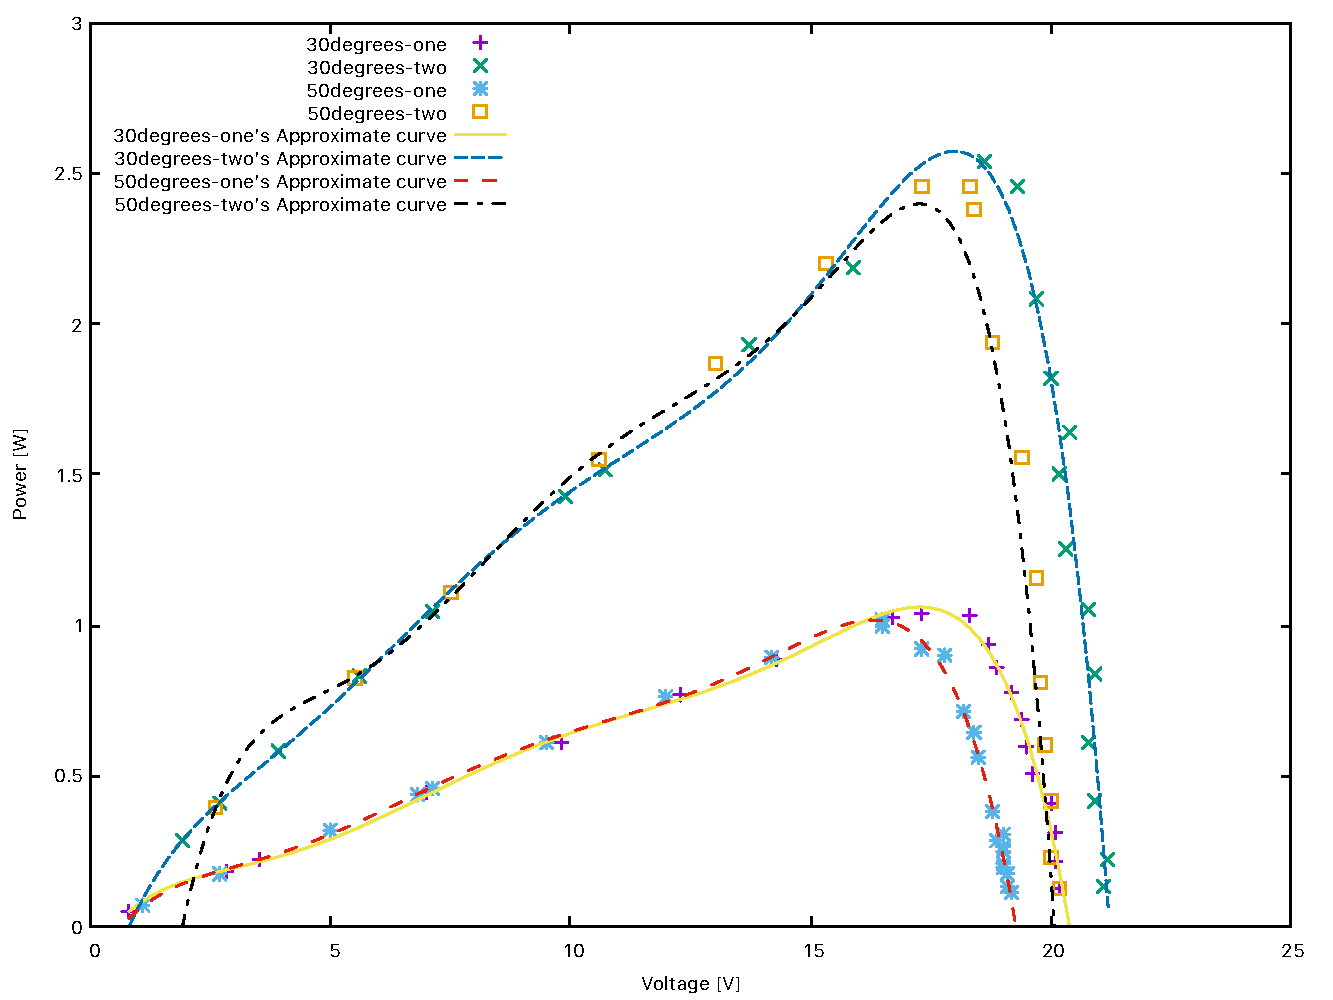
\includegraphics[scale=0.7]{./data/solar-cell/solar-cell-2.pdf}
	\caption{太陽電池の$V-P$カーブ}
	\label{fig:VPc}
	\end{minipage}
	\end{figure}
\end{itemize}

\clearpage
\subsubsection{太陽電池の発電特性の考察}
\begin{enumerate}[(1)]
	\item 各条件下の電流-電圧の測定結果から電力を算出し,$V-P$カーブを描きなさい.また,最大電力点を抽出して表にまとめ,条件の変化と最大電力点について考察せよ.
	
	$V-P$カーブは\wfig{VPc}に示した.\\
	最後に最大電流値を取る点が電力の最大点とほぼ一致していることが読み取れる.
	また,電力最大点より,小さい電圧の電流の傾きと.大きい電圧の電流の傾きは異なり,前者は緩やかで,後者は急である.
	電圧がある一定値を超えると急に電力を得ることが難しくなるとうことである.\\
	また,条件を変更しても電力最大点の移動が確認されなかったため,この点は太陽電池固有のものであると考えられる.$30^{\circ}$Cでライト2の場合つまり,低温で高い照度の場合が最も電力を多く得ることができている.\\
	電力は電流に比例し,\ref{solar-cell-result}で述べたように,より多くの電流ためにはより高い照度が必要であり,高温になると,低温時より,電力の低下がみられる.\\
	pn接合ダイオード電流は\weq{exp}で電流が算出できる.この式より,温度が増加すると電流が減少することが読み取れるため,上記の考察は正しいと考えられる.
	\item MPPT制御はなぜ必要か説明せよ.また,そのアルゴリズムには「山登り法」と「電圧追従法」がある.これらの特徴を調査し,比較して説明せよ.
	
	\wfig{VPc}の最大電力点で発電を行うように発電システムを構築したとしても,天候などの要因により電圧の増減し,電力が減少してしまう.そのため,最大電力点を用いた制御方法が必要となる.
	\begin{enumerate}
		\item[山登り法:] \wfig{mountan}の$P-V$曲線で電圧を一方向(増加または減少)に変化させていき,電力が増加から減少に転換すると電圧を変化させる方向を逆方向にする. これを繰り返すことにより,常に電力が最大となる最適動作点に制御する方法である\cite{esfvjsp}.
		最大電力出力点が山の頂に見え,山に登っていくように見えることからこの名前がついている.
		しかし,次に述べる電圧追従法より回路・制御が複雑であるため,コストや消費電力が高いという負の面もある\cite{nvdfsjknv}.
		\begin{figure}[h]
		\centering
		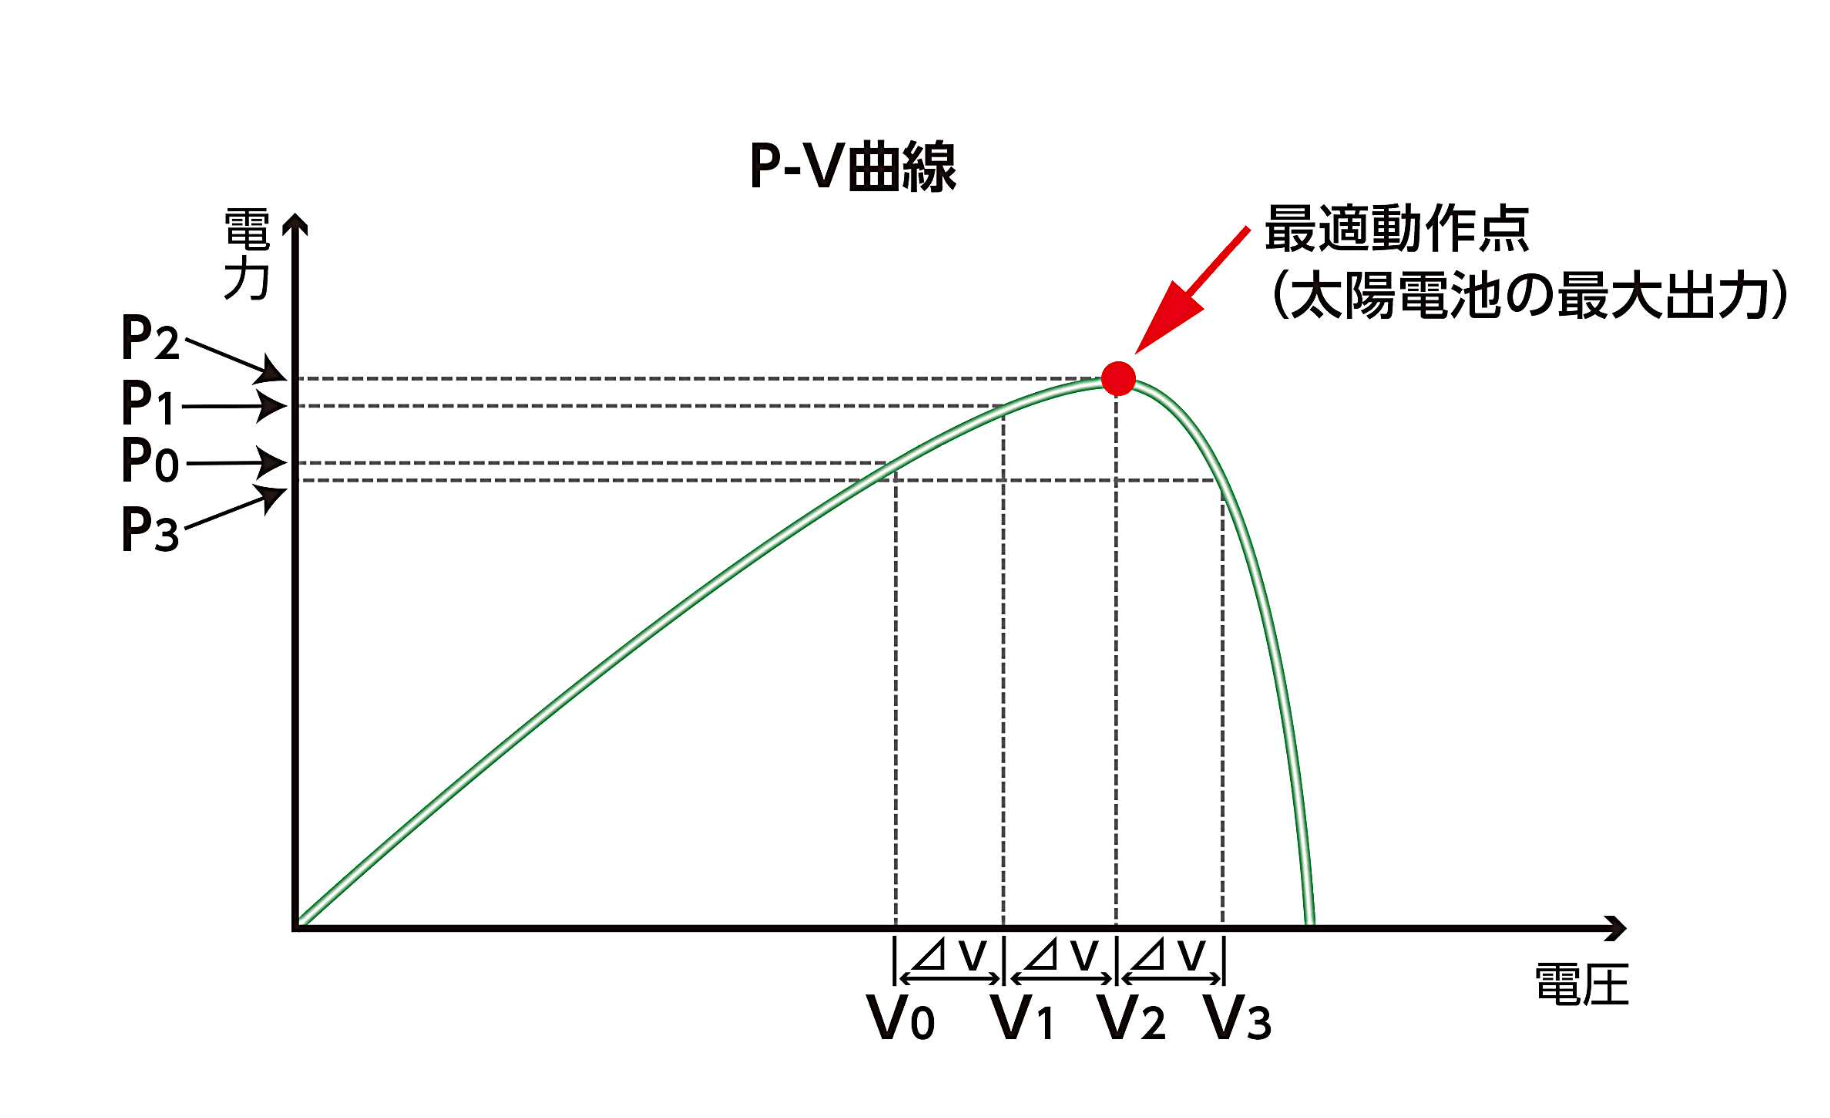
\includegraphics[scale=0.5]{./fig/mountan.png}
		\caption{山登り法\cite{esfvjsp}}
		\label{fig:mountan}
		\end{figure}
		\item[電圧追従法:]$V-I$出力特性を利用する方法である.\wfig{area}の枠の面積が発電電力を表し,$V1$のように発電電流が高く,$V2$のように発電電力が高くてもバランスが悪く,効率よく発電が行えていない状態である.しかし,$Vm$のようにそれぞれのバランスが良い状態の時,太陽電池は最大電力で発電が可能になる.この時の電圧値は開放電圧の約$80\,\%$である.
		太陽電池の動作点がバッテリーや負荷の電圧の影響を受けないため,一定の異常の効率で太陽電池から電力を取り出すことが可能である.また,電圧値の計測で制御が行えるため,容易で比較的安価であるが,気象条件により最適電圧が変動するため,最適電圧で動作していると言えない場合がある\cite{nvdfsjknv}.
		\begin{figure}[h]
		\centering
		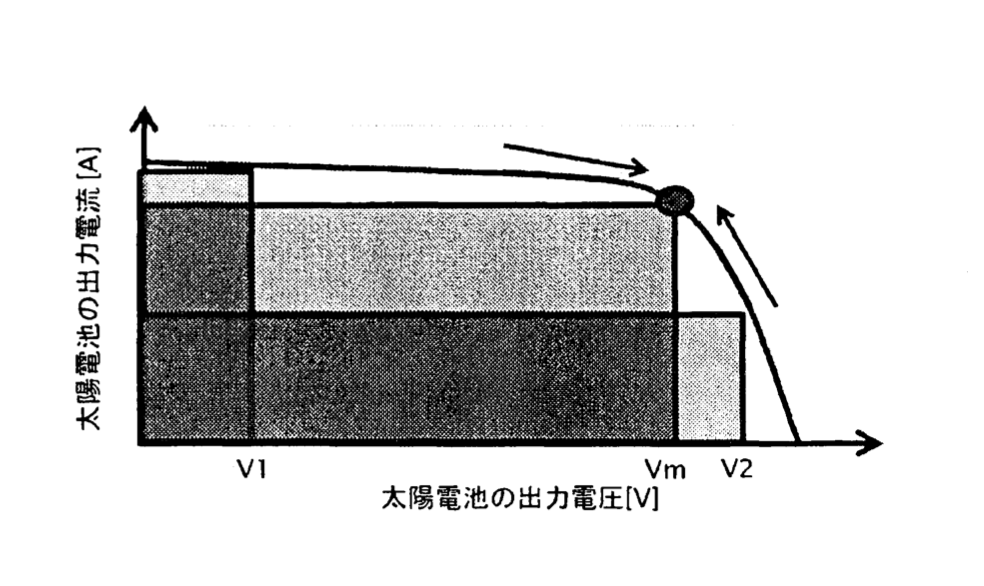
\includegraphics[scale=1]{./fig/area.png}
		\caption{電圧追従法\cite{nvdfsjknv}}
		\label{fig:area}
		\end{figure}
		\end{enumerate}
		なお,現在主流である制御方法は山登り法である\cite{main}.
\end{enumerate}

\clearpage
\section{結論}
この実験を通して,以下の点を達成することができた.
\begin{itemize}
	\item ダイオードの特性の1つである整流特性を実験により確認し,ダイオードを使用する
	\item ツェナーダイオード特性を理解し,利用する.
	\item 太陽電池の利用環境特性を知り,活用する.
\end{itemize}

\newpage
\printbibliography[title=参考文献]
\end{document}

